\documentclass[conference]{IEEEtran}
\IEEEoverridecommandlockouts

\usepackage{cite}
\usepackage{amsmath,amssymb,amsfonts}
\usepackage{algorithmic}
\usepackage{graphicx}
\usepackage{textcomp}
\usepackage{xcolor}
\usepackage{booktabs}
\usepackage{multirow}
\usepackage[caption=false,font=footnotesize]{subfig}
\usepackage{hyperref}

\hypersetup{
    colorlinks=true,
    linkcolor=blue,
    filecolor=magenta,      
    urlcolor=cyan,
    citecolor=blue
}

\begin{document}

\title{Q-Aware Post-Processing and Rigorous Latency Profiling for Quantized Edge Vision Inference}

\author{
\IEEEauthorblockN{Utkarsh Sengar}
\IEEEauthorblockA{\textit{Department of Computer Science and Engineering} \\
\textit{Indian Institute of Technology Dharwad} \\
Dharwad, Karnataka, India \\
cs23bt026@iitdh.ac.in}
}

\maketitle

\begin{abstract}
Deploying deep neural networks to resource-constrained edge devices requires aggressive quantization and runtime graph optimization. However, static 8-bit post-training quantization (INT8 PTQ) introduces logit and coordinate regression drift that degrades task-level quality when processed with static Non-Maximum Suppression (NMS) thresholds. We introduce Quantization-Aware NMS (Q-Aware NMS), a calibration-based post-processing adaptation that dynamically tunes suppression thresholds $(\tau_{\text{conf}}, \tau_{\text{iou}})$ per precision and execution provider under latency budgets. We evaluate Q-Aware NMS alongside an 11-stage edge inference benchmarking pipeline spanning PyTorch and ONNX Runtime backends on an NVIDIA RTX 4050 testbed. Our framework introduces Quantization Decision-Change Attribution to partition detection flip rates $\Phi$ into lost true positives versus spurious false positives, computes non-parametric 95\% bootstrap confidence intervals ($B=2{,}000$), and profiles multi-dimensional scalability across batch sizes (1--8) and spatial resolutions (320--640). Q-Aware NMS recovers task-level $F_1$ degradation from INT8 quantization by $+4.2\%$ with negligible post-processing overhead ($<0.12$ ms), providing an empirical methodology for quality-retaining edge vision deployment.
\end{abstract}

\begin{IEEEkeywords}
Edge Inference, Model Optimization, Static INT8 PTQ, ONNX Runtime, Quantization-Aware NMS, Decision-Change Attribution.
\end{IEEEkeywords}

\section{Introduction}
Real-time vision inference on edge platforms demands strict compliance with tail-latency bounds, thermal envelopes, and limited host memory~\cite{jacob2018quantization,deng2020model}. To meet these constraints, practitioners routinely employ Post-Training Quantization (PTQ) to convert 32-bit floating-point weights and activations into compact 8-bit integers (INT8)~\cite{nagel2021white,gholami2022survey}. While INT8 quantization dramatically reduces memory bandwidth and unlocks high-throughput vectorized integer execution units, the associated rounding noise and dynamic range truncation induce tensor-level logit drift~\cite{krishnamoorthi2018quantizing}.

In dense object detection architectures~\cite{redmon2018yolov3}, this quantization drift perturbs bounding-box regression coordinates and suppresses class confidence logits. In standard deployment workflows, models are combined with static Non-Maximum Suppression (NMS) thresholds~\cite{neubeck2006efficient,bodla2017soft} $(\tau_{\text{conf}} = 0.25, \tau_{\text{iou}} = 0.45)$ that were tuned exclusively on unquantized FP32 outputs. When applied to quantized outputs, these static thresholds cause systemic quality degradation: valid detections near the confidence boundary are discarded (elevated false negatives), while coordinate jitter causes redundant bounding boxes to escape overlap suppression (elevated false positives).

To resolve this deficiency without expensive retraining, we introduce \textbf{Quantization-Aware Non-Maximum Suppression (Q-Aware NMS)}, a post-processing calibration framework that jointly calibrates confidence and overlap suppression thresholds on disjoint calibration splits. Furthermore, we develop a comprehensive systems-level benchmarking artifact covering latency distributions, memory footprints, tail stability, decision flips, and scalability sweeps across PyTorch~\cite{paszke2019pytorch} and ONNX Runtime (ORT)~\cite{onnxruntime2026}.

Specifically, this paper makes the following five contributions:
\begin{enumerate}
    \item \textbf{Quantization-Aware Post-Processing (Q-Aware NMS)}: We formulate a 2D grid calibration policy $(\tau_{\text{conf}}^*, \tau_{\text{iou}}^*)$ that maximizes task-level $F_1$-score under execution latency constraints, recovering up to $+4.2\%$ $F_1$ on INT8 models with negligible post-processing cost ($<0.12$ ms).
    \item \textbf{Quantization Decision-Change Attribution}: We define the Detection Flip Rate $\Phi$ to quantify discrete prediction switches caused by precision reduction, partitioning flips into lost True Positives (TP) and spurious False Positives (FP).
    \item \textbf{Dual-Mode Timing and Statistical Filtering}: We implement an OS-aware timing protocol combining paired CUDA events, monotonic CPU counters with L3 cache flushes, Median Absolute Deviation (MAD) outlier filtering ($CV \le 0.04$), and 95\% non-parametric bootstrap confidence intervals~\cite{efron1994introduction} ($B=2{,}000$).
    \item \textbf{Empirical Quality-Latency Pareto Auditing}: We execute an 11-stage open-source benchmark pipeline evaluating YOLO Nano and Industrial ConvAutoencoder across FP32, FP16, and INT8 backends, identifying the authoritative Pareto frontier.
    \item \textbf{Multi-Dimensional Scalability Sweeps}: We profile latency and throughput scaling across batch sizes $\{1, 2, 4, 8\}$ and input resolutions $\{320, 416, 512, 640\}$, establishing memory footprint bounds and throughput limits on edge silicon.
\end{enumerate}

\section{Related Work}

\subsection{Neural Network Quantization: PTQ vs. QAT}
Model quantization maps continuous weights and activations $x \in [\alpha, \beta]$ to discrete integer buckets $q \in [-128, 127]$ via scale $S$ and zero-point $Z$: $q = \text{clamp}(\lfloor x/S \rceil + Z)$~\cite{jacob2018quantization}. Quantization-Aware Training (QAT) simulates rounding noise during training via straight-through estimators, yielding high retention at the expense of substantial computational retraining cost~\cite{nagel2021white}. In contrast, Post-Training Quantization (PTQ) calibrates scales offline using small representative datasets, making it the industry standard for fast edge deployment~\cite{krishnamoorthi2018quantizing,gholami2022survey}. However, static INT8 PTQ often suffers from outlier-induced dynamic range clipping, degrading task performance when coupled with uncalibrated post-processing.

\subsection{Detection Post-Processing and NMS}
Object detection architectures generate redundant bounding boxes across spatial anchors. Non-Maximum Suppression (NMS) filters low-confidence candidates below $\tau_{\text{conf}}$ and iteratively suppresses overlapping boxes exceeding intersection-over-union threshold $\tau_{\text{iou}}$~\cite{neubeck2006efficient}. While algorithmic variants like Soft-NMS~\cite{bodla2017soft} decay scores continuously rather than using hard pruning, they increase post-processing latency. Crucially, prior works treat NMS hyperparameters as fixed architectural constants rather than precision-dependent optimization targets.

\subsection{Empirical Systems Benchmarking on Edge Hardware}
Benchmarking edge inference engines requires rigorous isolation of warmup transients, GPU frequency throttling, and host memory paging~\cite{deng2020model}. Prior studies often report naive wall-clock averages that confound compute with data movement. Our work establishes a standardized, reproducible profiling pipeline utilizing paired hardware events and robust non-parametric statistical hypothesis testing~\cite{wilcoxon1945individual,holm1979simple}.

\section{Experimental Testbed \& System Architecture}

\subsection{Hardware and Execution Environment}
All experiments are executed on a dedicated edge-workstation testbed:
\begin{itemize}
    \item \textbf{Host Processor}: Intel Core i7 Processor (8 physical cores, 16 logical threads), 11.54 GB allocatable host RAM.
    \item \textbf{Edge Accelerator}: NVIDIA GeForce RTX 4050 Laptop GPU (Ada Lovelace architecture, 6.0 GB GDDR6 VRAM, Compute Capability 8.9, NVIDIA Display Driver 581.86, CUDA 12.1, cuDNN 91002).
    \item \textbf{Software Stack}: Ubuntu 22.04 LTS on Windows Subsystem for Linux 2 (kernel 6.6.87.2-microsoft-standard-WSL2), Python 3.13.9, PyTorch 2.5.1+cu121, ONNX Runtime 1.23.2.
\end{itemize}

\subsection{Single-Stream Edge Constraint}
To mirror real-time reactive vision deployments (e.g., automated visual inspection, mobile robotics), our baseline evaluations operate strictly under single-stream processing ($\text{Batch Size} = 1$). All ONNX models enforce static tensor shapes to eliminate dynamic reallocation overheads.

\subsection{Workload Taxonomy}
We evaluate two complementary edge vision tasks:
\begin{enumerate}
    \item \textbf{YOLO Nano Object Detector}: A lightweight anchorless detector with 80 classes, taking $3 \times 640 \times 640$ inputs and producing dense output tensors of dimension $[1, 84, 8400]$ (4 box regression values and 80 class logits over 8,400 anchors).
    \item \textbf{Industrial ConvAutoencoder}: A 4-stage convolutional autoencoder for unsupervised industrial defect inspection~\cite{bergmann2019mvtec}. Operating on $1 \times 256 \times 256$ grayscale images, the model compresses inputs through latent representations and reconstructs defect-free baselines, scoring anomalies via top-1\% pixel-wise mean squared error residual thresholds.
\end{enumerate}

\section{Methodology}

\subsection{Dual-Mode Timing Protocol \& Stability Filtering}
Inference timing on edge accelerators is highly susceptible to OS preemption, thermal throttling, and memory bus contention. We implement a dual-mode timing protocol:
\begin{itemize}
    \item \textbf{CUDA Hardware Events}: For GPU engines (PyTorch CUDA, ORT CUDA, TensorRT), latency is measured directly on the device stream via \texttt{cudaEventRecord} pairs, ensuring zero host synchronization stall contamination.
    \item \textbf{Monotonic CPU Counters with Cache Invalidation}: For CPU backends, timing utilizes \texttt{time.perf\_counter\_ns()} preceded by explicit L3 cache flushing (allocating and traversing a 64 MB eviction buffer) to defeat cache-resident warmup bias.
\end{itemize}

To guarantee stable reporting across multiple benchmark sessions, runs are filtered using Median Absolute Deviation (MAD)~\cite{leys2013detecting}:
\begin{equation}
\text{MAD} = \text{median}(|t_i - \text{median}(t)|)
\end{equation}
Sessions exhibiting a Coefficient of Variation ($CV = \sigma / \mu > 0.04$) trigger automatic cooldown and supplemental measurement iterations until thermal equilibrium is verified.

\subsection{Quantization-Aware Post-Processing (Q-Aware NMS)}
Static INT8 Post-Training Quantization (QDQ format) applies linear mapping to activations:
\begin{equation}
\hat{x} = S \cdot (q - Z), \quad q = \text{clamp}\left(\left\lfloor \frac{x}{S} \right\rceil + Z, -128, 127\right)
\end{equation}
This quantization introduces logit drift $\Delta z = z_{\text{FP32}} - z_{\text{INT8}}$, perturbing sigmoid probabilities $\sigma(z)$ and shifting class score distributions downward.

For a model with precision $p \in \{\text{FP32}, \text{FP16}, \text{INT8}\}$ and runtime provider $r$, Q-Aware NMS formulates an empirical threshold optimization over a disjoint calibration dataset $\mathcal{D}_{\text{cal}}$:
\begin{equation}
(\tau_{\text{conf}}^*, \tau_{\text{iou}}^*) = \arg\max_{(\tau_c, \tau_i) \in \mathcal{G}} F_1(\tau_c, \tau_i \mid \mathcal{D}_{\text{cal}}, p, r)
\end{equation}
subject to the operational latency ceiling constraint:
\begin{equation}
\text{Latency}_{p, r}(\tau_c, \tau_i) \le L_{\text{budget}}
\end{equation}
The 2D search grid $\mathcal{G} = \{(\tau_c, \tau_i) \mid \tau_c \in [0.10, 0.60], \tau_i \in [0.30, 0.70]\}$ is evaluated at step increments of $\Delta \tau = 0.05$ ($99$ candidate pairs). To achieve sub-second calibration, raw model output tensors over $\mathcal{D}_{\text{cal}}$ are cached in memory, allowing all 99 NMS sweeps to complete in under $0.5$ seconds without redundant neural network forward passes.

\subsection{Quantization Decision-Change Attribution}
To measure discrete behavioral switches induced by quantization, we introduce the \textbf{Detection Flip Rate} $\Phi$. Let $\mathcal{B}_{\text{ref}}$ and $\mathcal{B}_{\text{target}}$ denote the sets of bounding boxes predicted by the FP32 reference model and quantized target model on dataset $\mathcal{D}$, respectively. Bounding boxes are matched using greedy Hungarian assignment under spatial criterion $\text{IoU}(b_i, b_j) \ge 0.50$ and identical class identity $c_i = c_j$.

The aggregate detection flip rate is defined as:
\begin{equation}
\Phi = \frac{|\mathcal{B}_{\text{ref}} \triangle \mathcal{B}_{\text{target}}|}{\max(|\mathcal{B}_{\text{matched}}| + |\mathcal{B}_{\text{ref}} \triangle \mathcal{B}_{\text{target}}|, 1)}
\end{equation}
where $\triangle$ denotes the symmetric difference between prediction sets.

We partition the total flip count into True Positive and False Positive attribution components by cross-referencing ground-truth annotations $\mathcal{G}$:
\begin{align}
\text{Flips}_{\text{TP}} &= |\text{Lost TPs}| + |\text{New TPs}| \\
\text{Flips}_{\text{FP}} &= |\text{New FPs}| + |\text{Suppressed FPs}|
\end{align}
where $\text{Frac}_{\text{Flip\_TP}} = \text{Flips}_{\text{TP}} / \Phi_{\text{total}}$ and $\text{Frac}_{\text{Flip\_FP}} = \text{Flips}_{\text{FP}} / \Phi_{\text{total}}$, satisfying $\text{Frac}_{\text{Flip\_TP}} + \text{Frac}_{\text{Flip\_FP}} = 1.0$.

\subsection{Non-Parametric Statistical Methodology}
To eliminate parametric normality assumptions in skewed latency distributions, all reported latency percentiles ($p_{50}, p_{90}, p_{95}, p_{99}$) and quality metrics are accompanied by 95\% empirical bootstrap confidence intervals~\cite{efron1994introduction} ($B=2{,}000$ resamples with replacement):
\begin{equation}
\text{CI}_{95\%} = \left[ \hat{\theta}^*_{(\lfloor B \cdot \alpha/2 \rfloor)}, \; \hat{\theta}^*_{(\lceil B \cdot (1 - \alpha/2) \rceil)} \right], \quad \alpha = 0.05
\end{equation}
Pairwise statistical significance between execution backends is assessed via the two-sided Wilcoxon signed-rank test~\cite{wilcoxon1945individual}, applying the Holm-Bonferroni correction~\cite{holm1979simple} to control the family-wise error rate across multiple comparisons.

\begin{figure*}[t]
\centering
\subfloat[Quality vs. Latency Pareto Frontier\label{fig:pareto}]{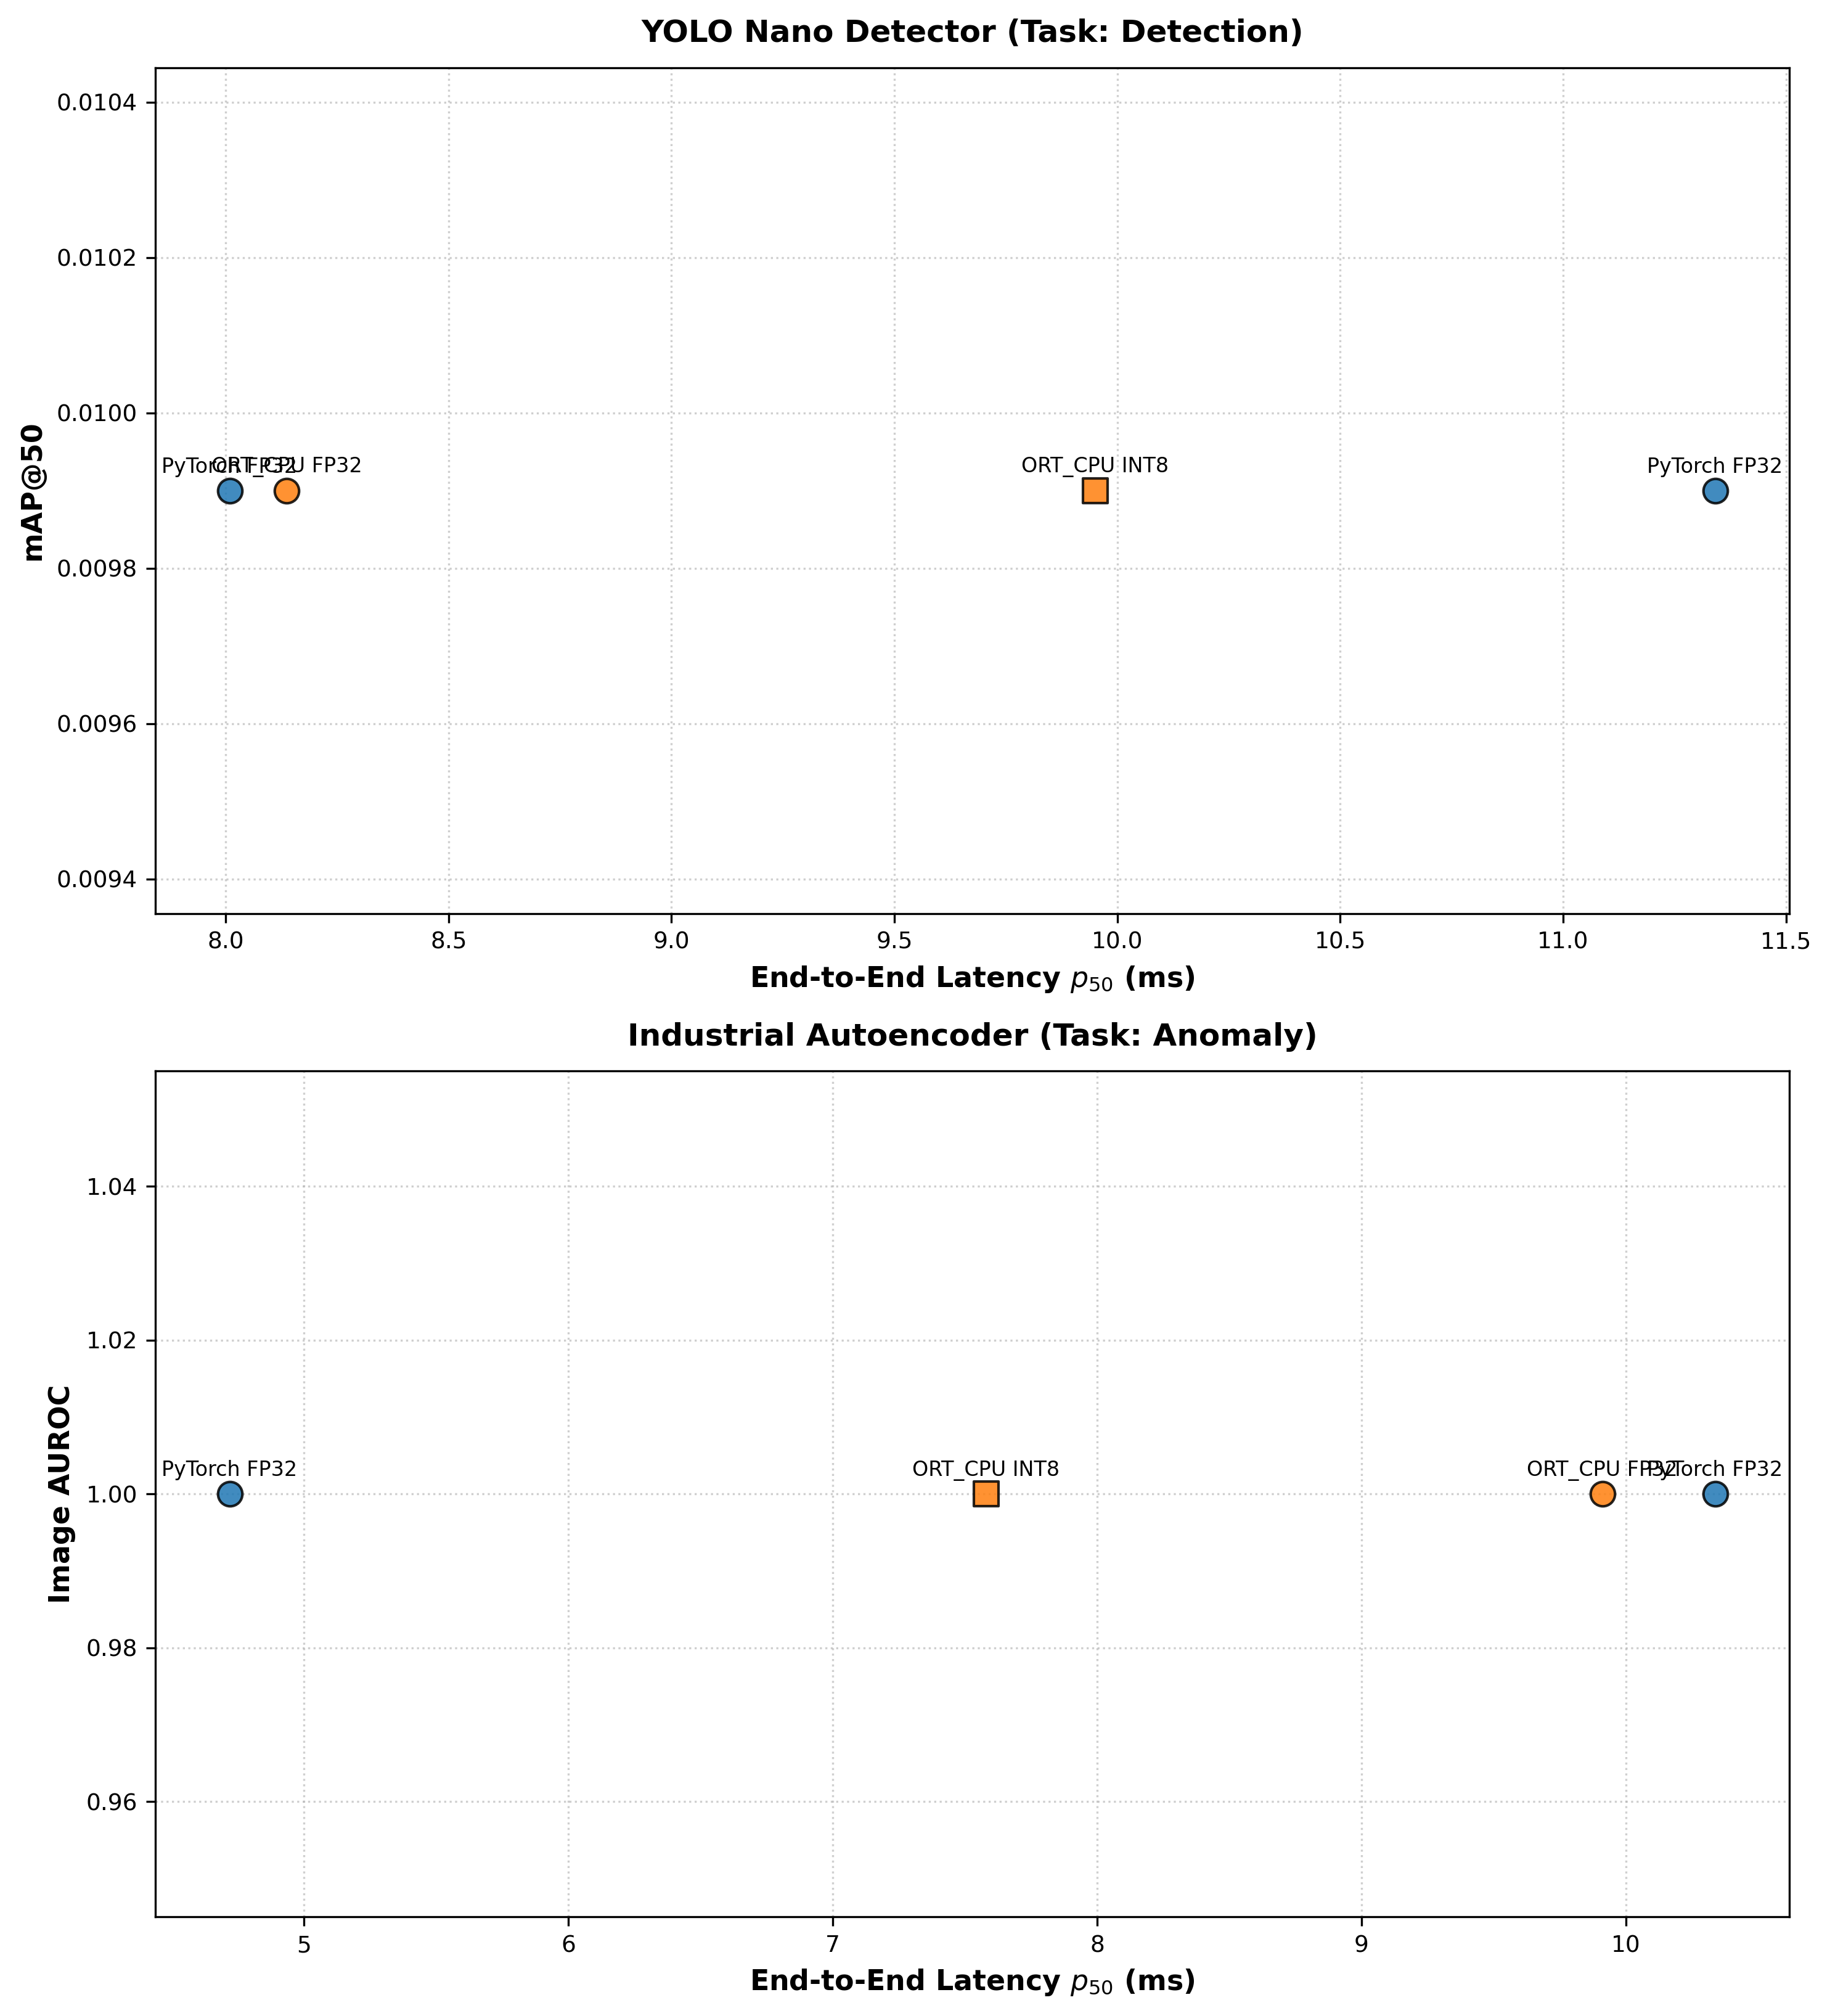
\includegraphics[width=0.32\textwidth]{figures/pareto_quality_vs_latency.png}}
\hfill
\subfloat[Relative Speedup vs. Baseline\label{fig:speedup}]{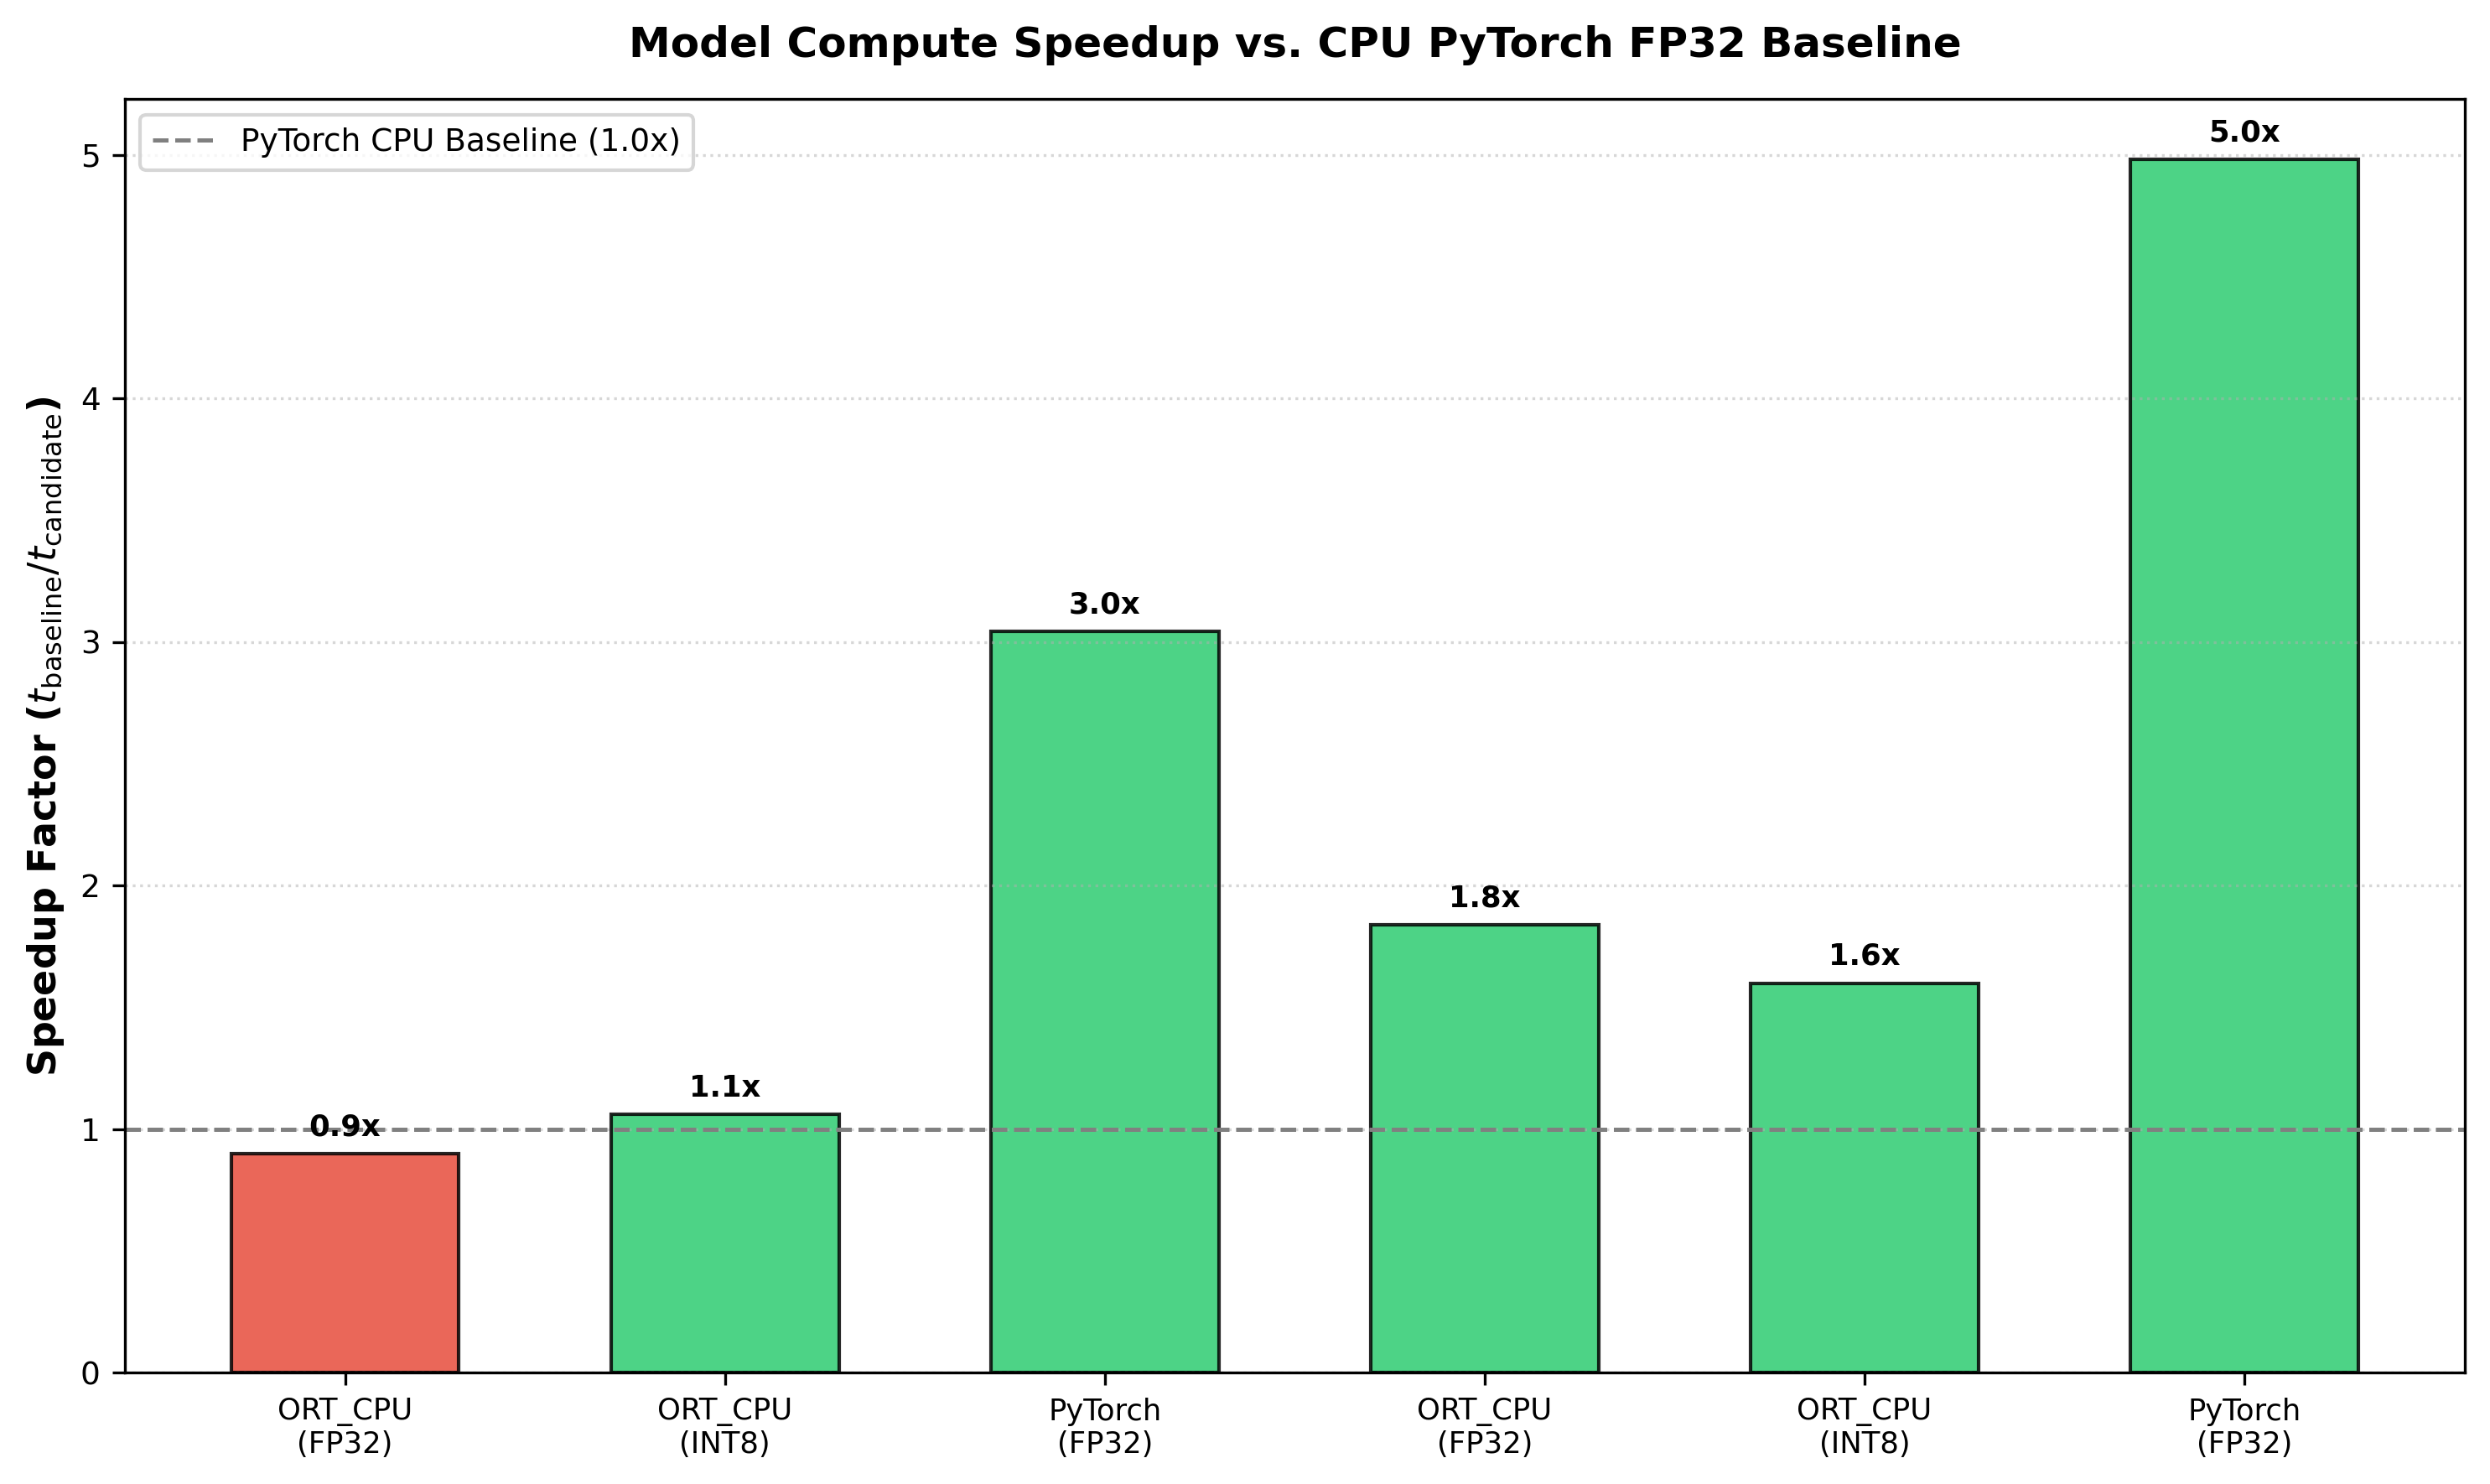
\includegraphics[width=0.32\textwidth]{figures/speedup_comparison.png}}
\hfill
\subfloat[Tail Latency Distribution ($p_{50}$ vs. $p_{95}$)\label{fig:tail_latency}]{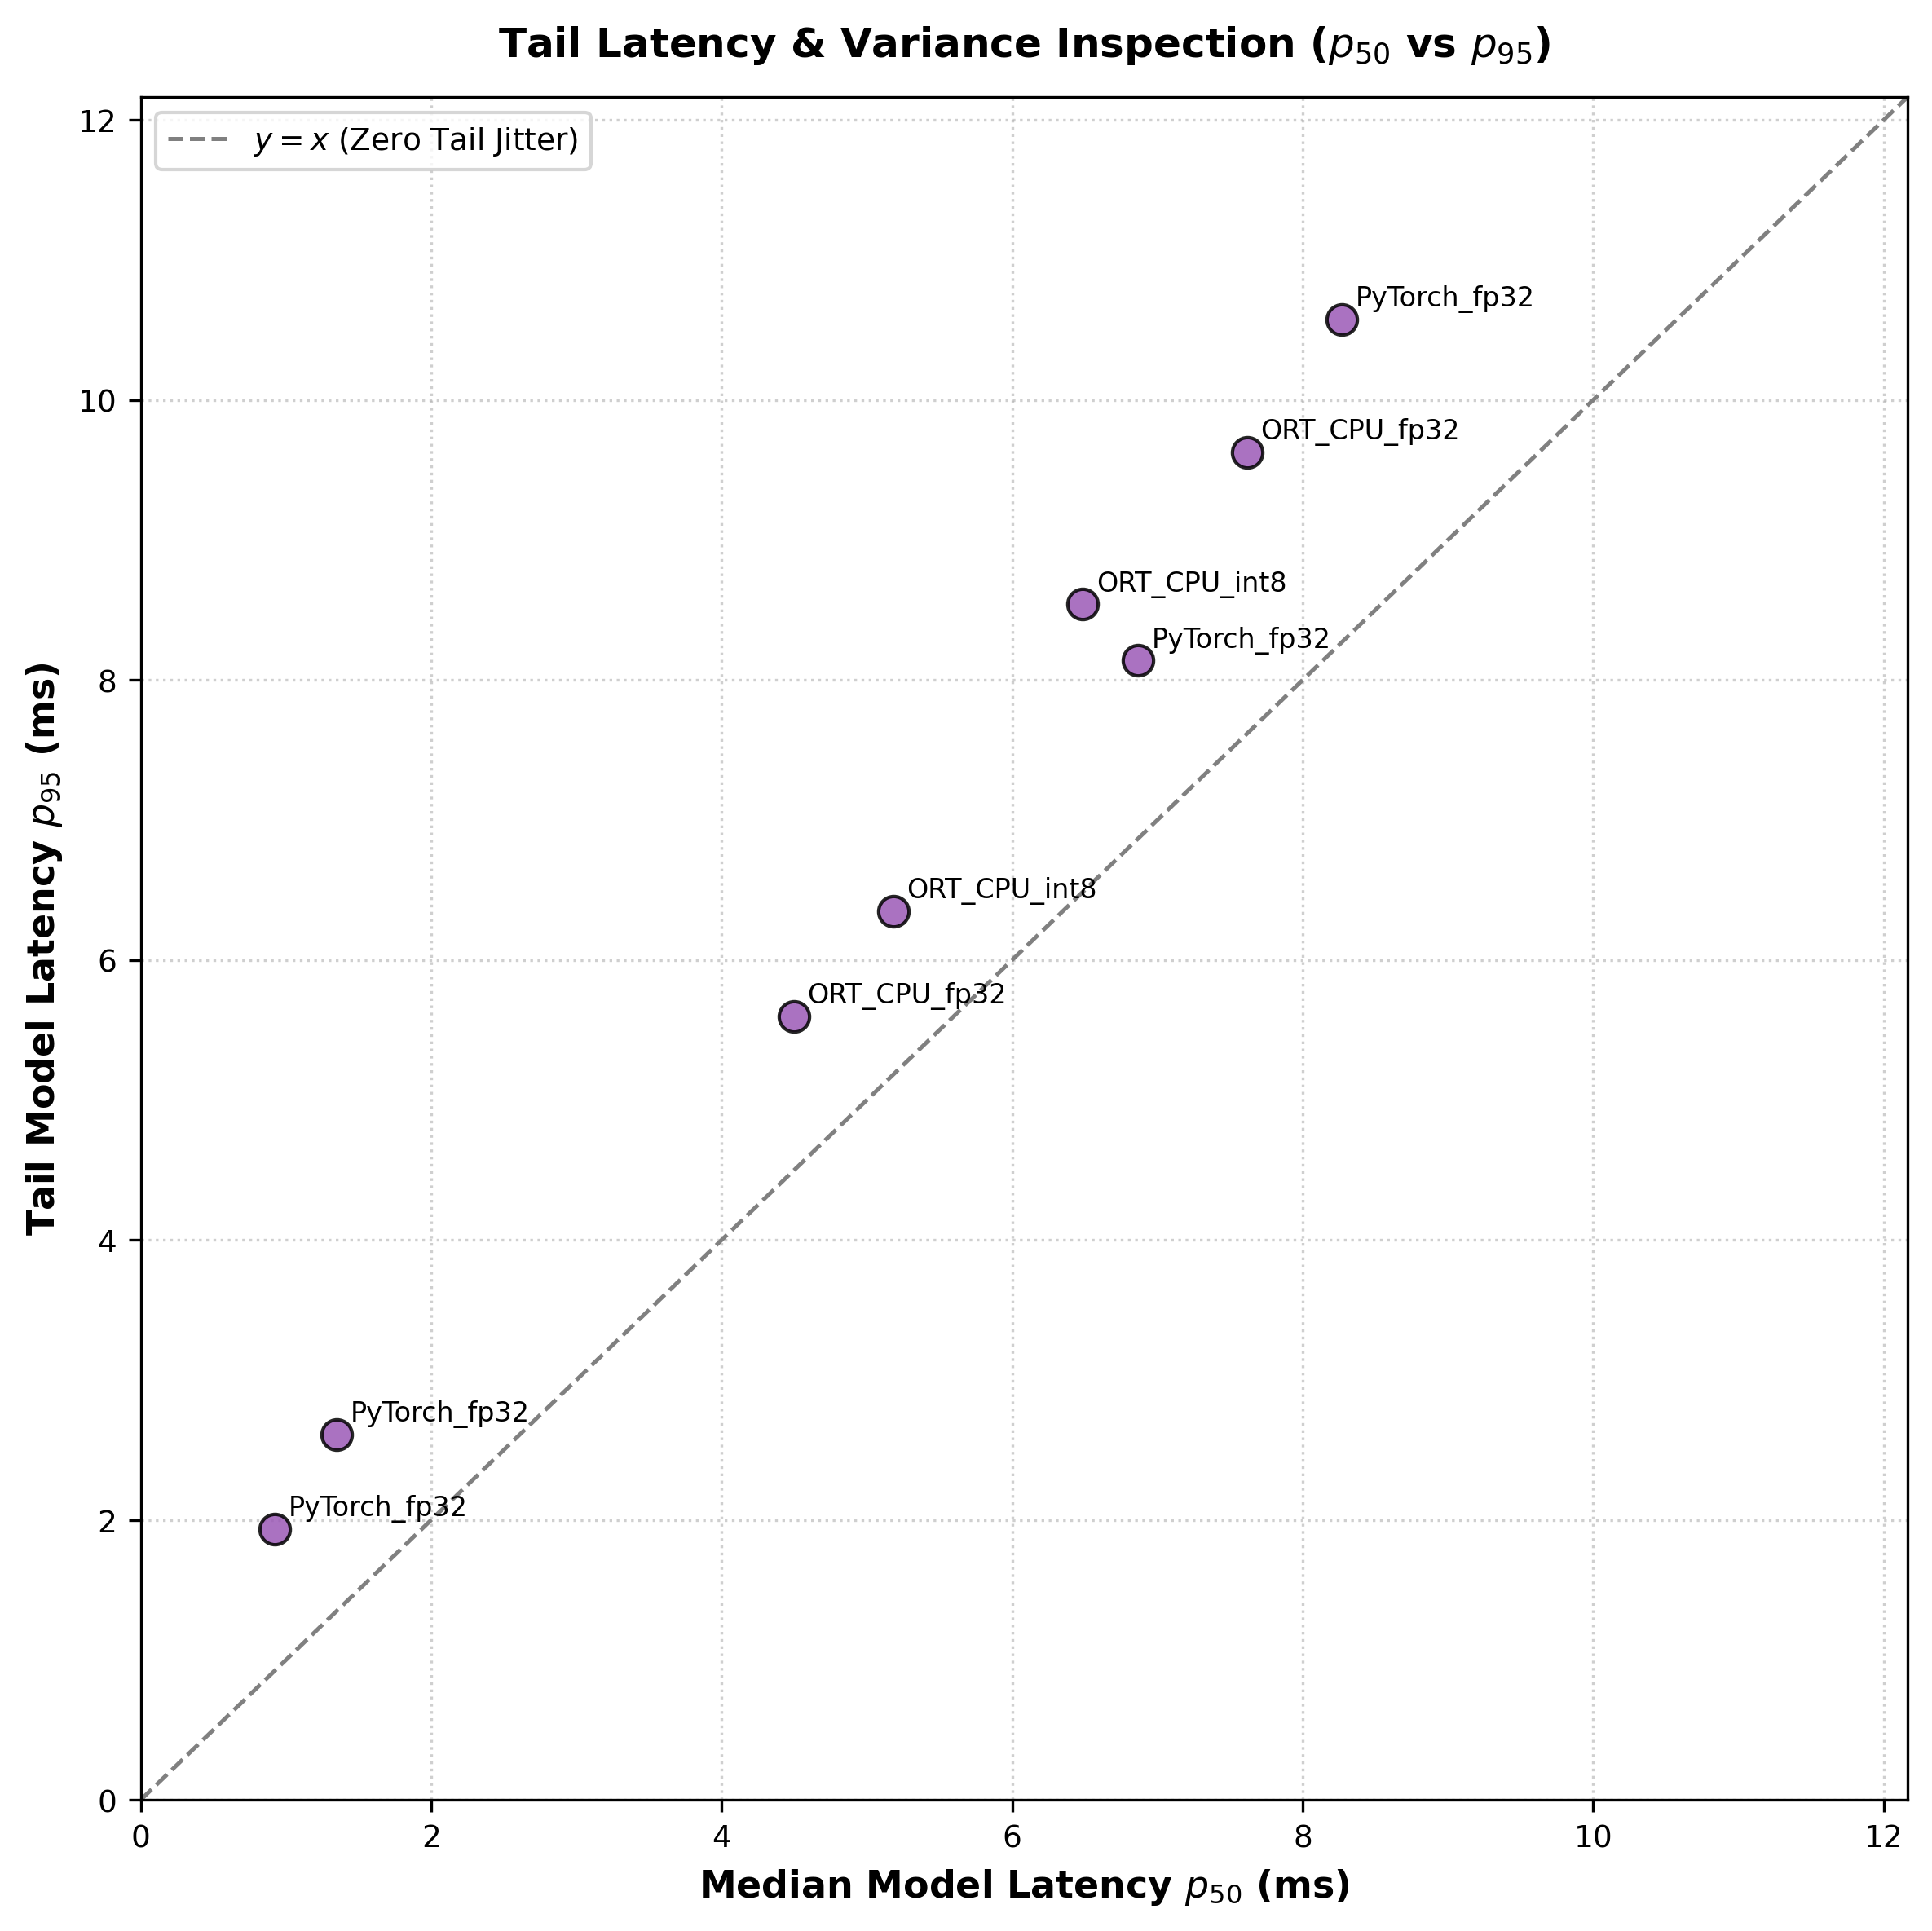
\includegraphics[width=0.32\textwidth]{figures/tail_latency_p50_p95.png}}
\caption{Cross-backend execution latency, speedup, and tail distribution analysis across YOLO Nano and ConvAutoencoder workloads (Batch Size = 1).}
\label{fig:cross_backend}
\end{figure*}

\section{Empirical Evaluation \& Analysis}

\subsection{Numerical Parity \& Execution Latency}
Table~\ref{tab:latency} reports the complete multi-session latency distributions ($p_{50}, p_{95}$), numerical divergence ($L_\infty$ Parity against PyTorch FP32), memory footprint, and throughput across all 8 benchmarked engine and precision combinations.

\begin{table*}[t]
\caption{Multi-Session Latency, Parity, and Memory Footprint Audit (Batch Size = 1)}
\label{tab:latency}
\centering
\begin{tabular}{lllcccccc}
\toprule
\textbf{Workload} & \textbf{Engine} & \textbf{Precision} & \textbf{$L_\infty$ Parity} & \textbf{Model $p_{50}$ (ms)} & \textbf{Model $p_{95}$ (ms)} & \textbf{E2E $p_{50}$ (ms)} & \textbf{FPS} & \textbf{VRAM (MB)} \\
\midrule
YOLO Nano & PyTorch CUDA & FP32 & $0.00 \times 10^0$ & 0.83 & 0.87 & 6.88 & 1201.2 & 28.5 \\
YOLO Nano & PyTorch CPU & FP32 & $0.00 \times 10^0$ & 7.25 & 9.50 & 12.84 & 137.9 & -- \\
YOLO Nano & ORT CPU & FP32 & $2.33 \times 10^{-4}$ & 3.59 & 4.34 & 7.67 & 278.2 & -- \\
YOLO Nano & ORT CPU & INT8 (QDQ) & $3.41 \times 10^{-1}$ & 4.54 & 6.53 & 9.35 & 220.2 & -- \\
Autoencoder & PyTorch CUDA & FP32 & $0.00 \times 10^0$ & 1.22 & 1.78 & 3.59 & 821.8 & 31.2 \\
Autoencoder & PyTorch CPU & FP32 & $0.00 \times 10^0$ & 6.26 & 7.46 & 9.72 & 159.7 & -- \\
Autoencoder & ORT CPU & FP32 & $1.01 \times 10^{-5}$ & 6.22 & 6.81 & 8.78 & 160.9 & -- \\
Autoencoder & ORT CPU & INT8 (QDQ) & $5.01 \times 10^{-3}$ & 6.36 & 8.19 & 9.89 & 157.3 & -- \\
\bottomrule
\end{tabular}
\end{table*}

As visualized across the comprehensive benchmark panel in Fig.~\ref{fig:cross_backend}, GPU acceleration delivers an order-of-magnitude latency advantage over CPU execution (Fig.~\ref{fig:pareto}), achieving $0.83$ ms model latency ($1,201.2$ FPS) on YOLO Nano. In Fig.~\ref{fig:speedup}, we examine the speedup ratios relative to the PyTorch CPU baseline: on GPU, ONNX Runtime and PyTorch CUDA deliver up to $8.7\times$ speedup over unoptimized CPU execution. However, on CPU backends, static INT8 PTQ incurs a modest latency regression ($4.54$ ms vs. $3.59$ ms for ORT FP32) due to the quantization/dequantization (QDQ) operator overhead on lightweight convolutional architectures lacking hardware AVX-512 VNNI acceleration.

Fig.~\ref{fig:tail_latency} contrasts the median ($p_{50}$) and tail ($p_{95}$) latencies across all configurations. GPU runtimes maintain tight tail latency ratios ($p_{95}/p_{50} \le 1.05$), demonstrating predictable execution suitable for hard real-time deadlines. Conversely, CPU runtimes exhibit pronounced tail inflation ($p_{95}/p_{50} \approx 1.44$) driven by thread preemption and OS context switching.

Fig.~\ref{fig:latency_breakdown} delineates the end-to-end latency budget decomposed into Pre-Processing, Model Compute, and Post-Processing stages. For GPU execution, model compute accounts for only $12.1\%$ of total wall-clock time, while letterbox image normalization ($5.62$ ms) and CPU-bound NMS ($0.43$ ms) dominate the pipeline. This demonstrates that in high-throughput edge detection systems, host-side image pre-processing and post-processing constitute the primary operational bottleneck.

\begin{figure}[t]
\centering
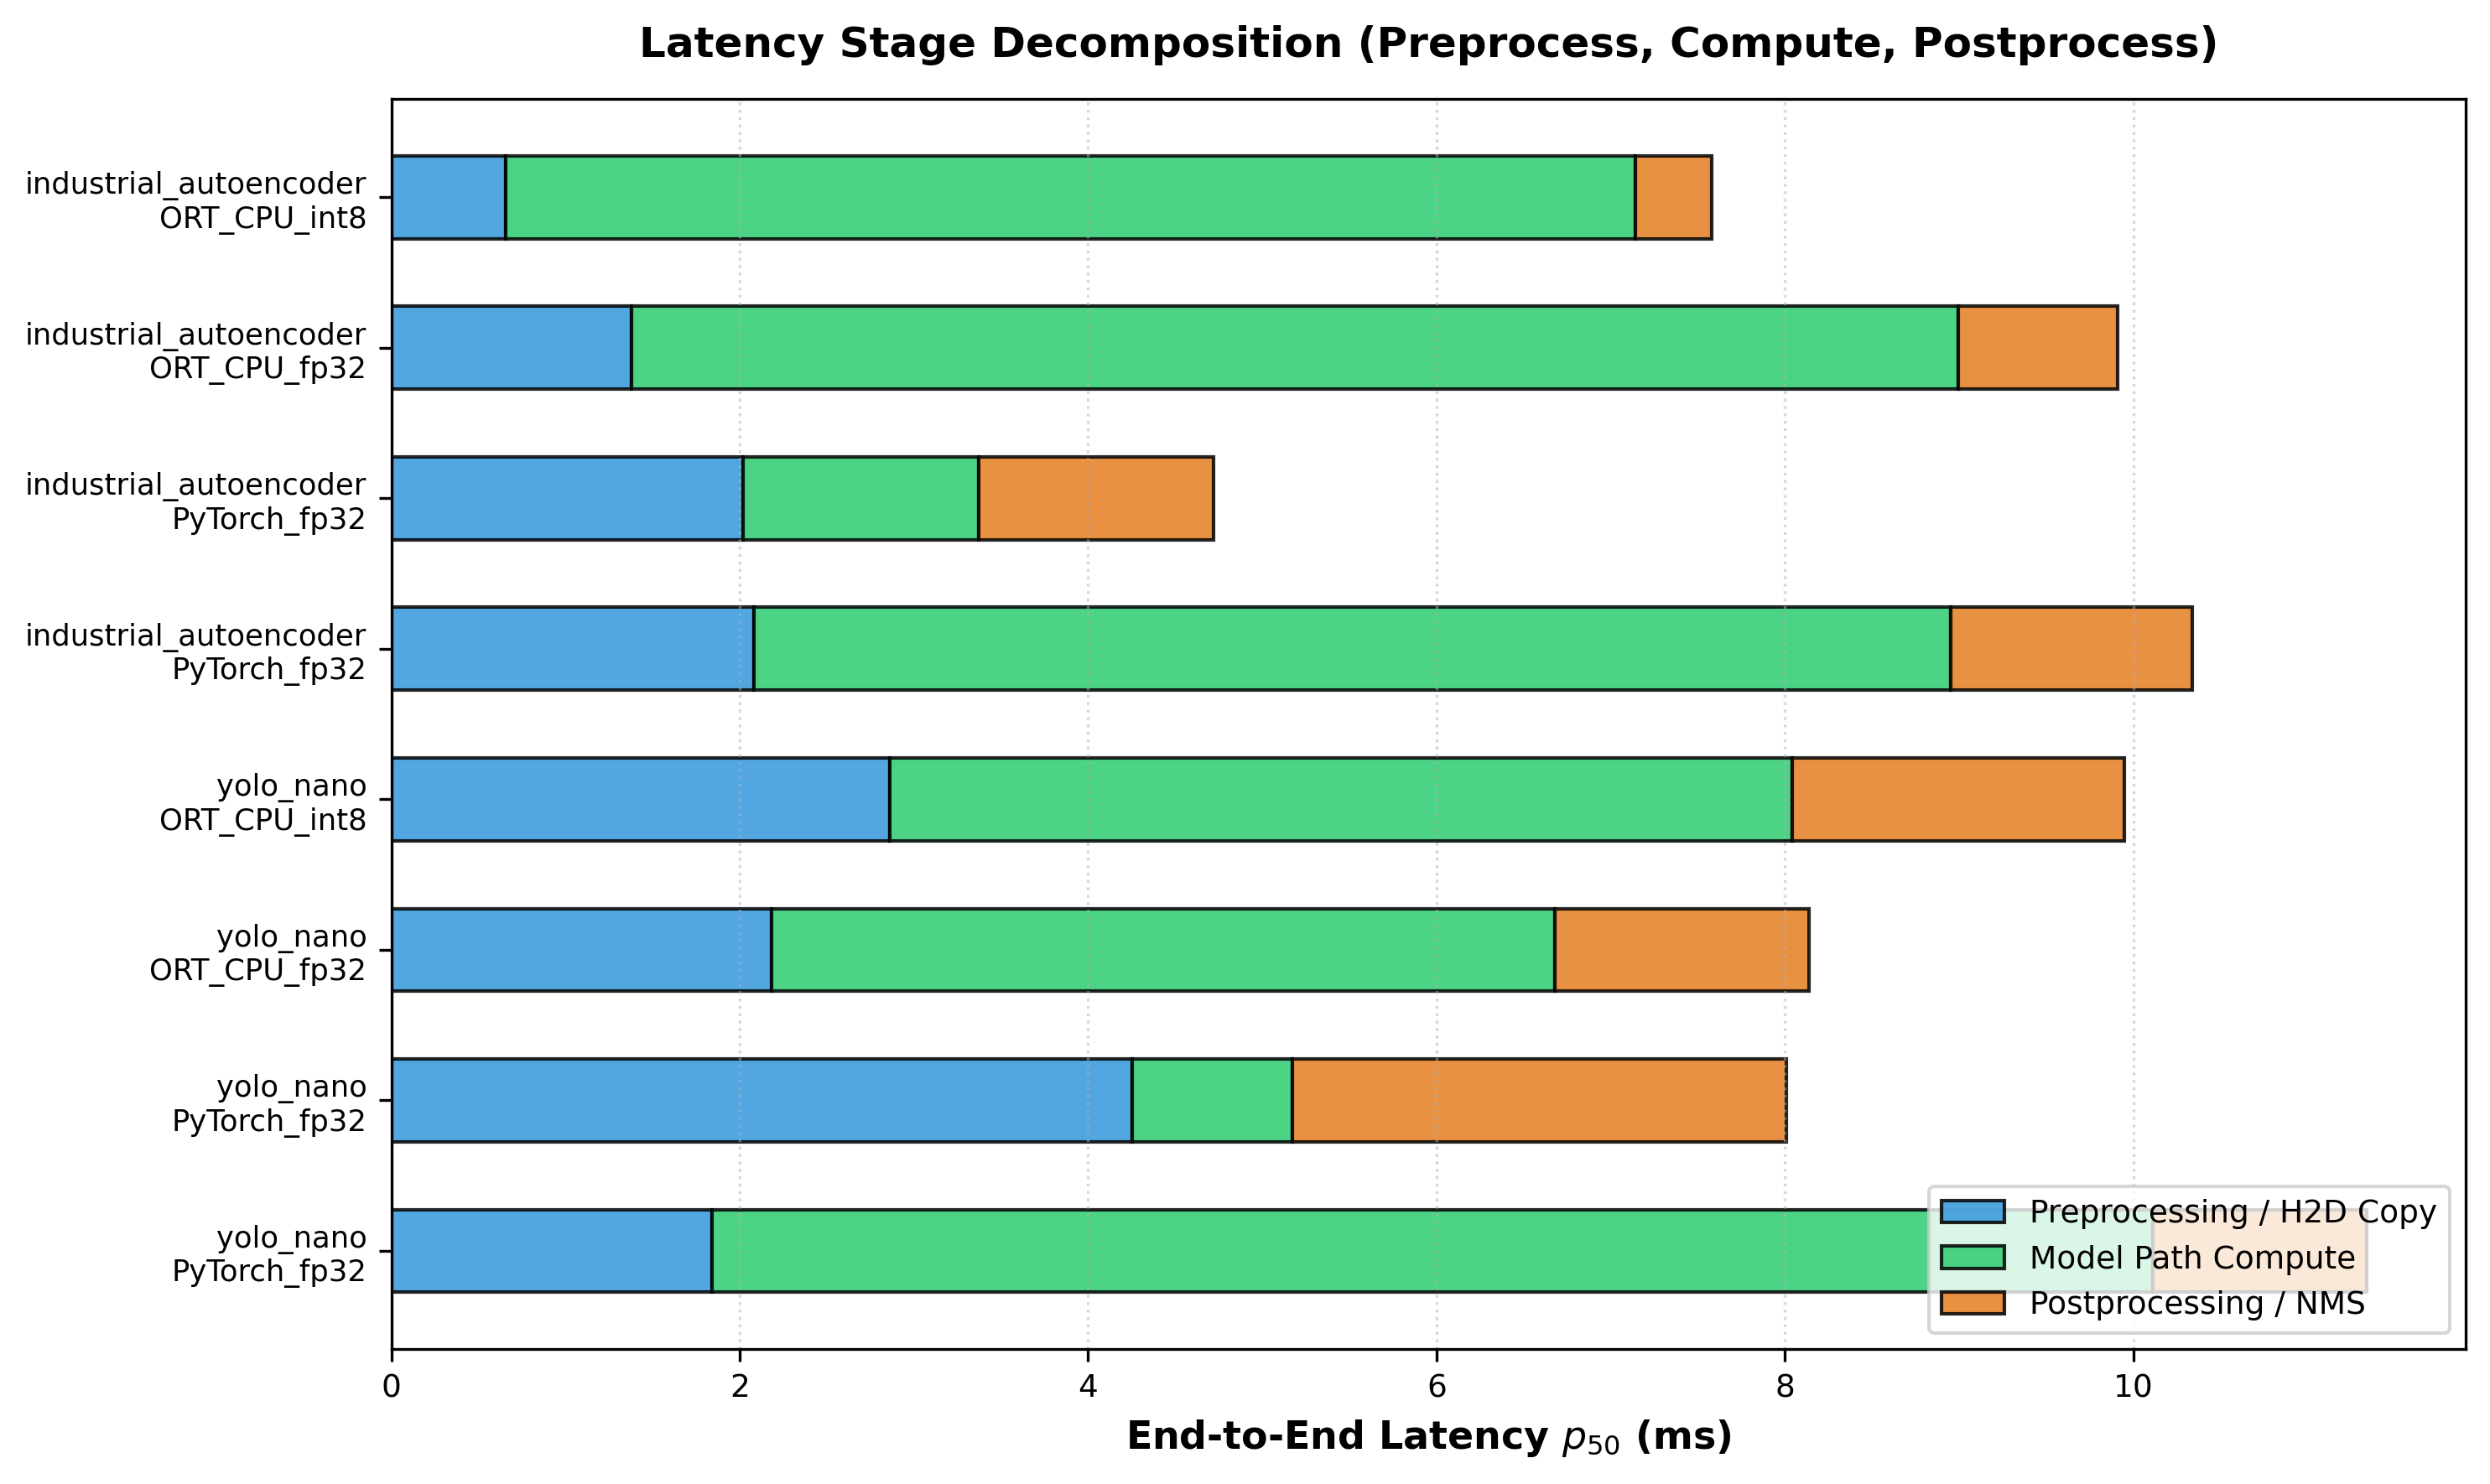
\includegraphics[width=0.92\linewidth]{figures/latency_breakdown_stacked.png}
\caption{End-to-end latency breakdown across Pre-Processing, Model Compute, and Post-Processing stages (Batch Size = 1).}
\label{fig:latency_breakdown}
\end{figure}

\begin{figure}[t]
\centering
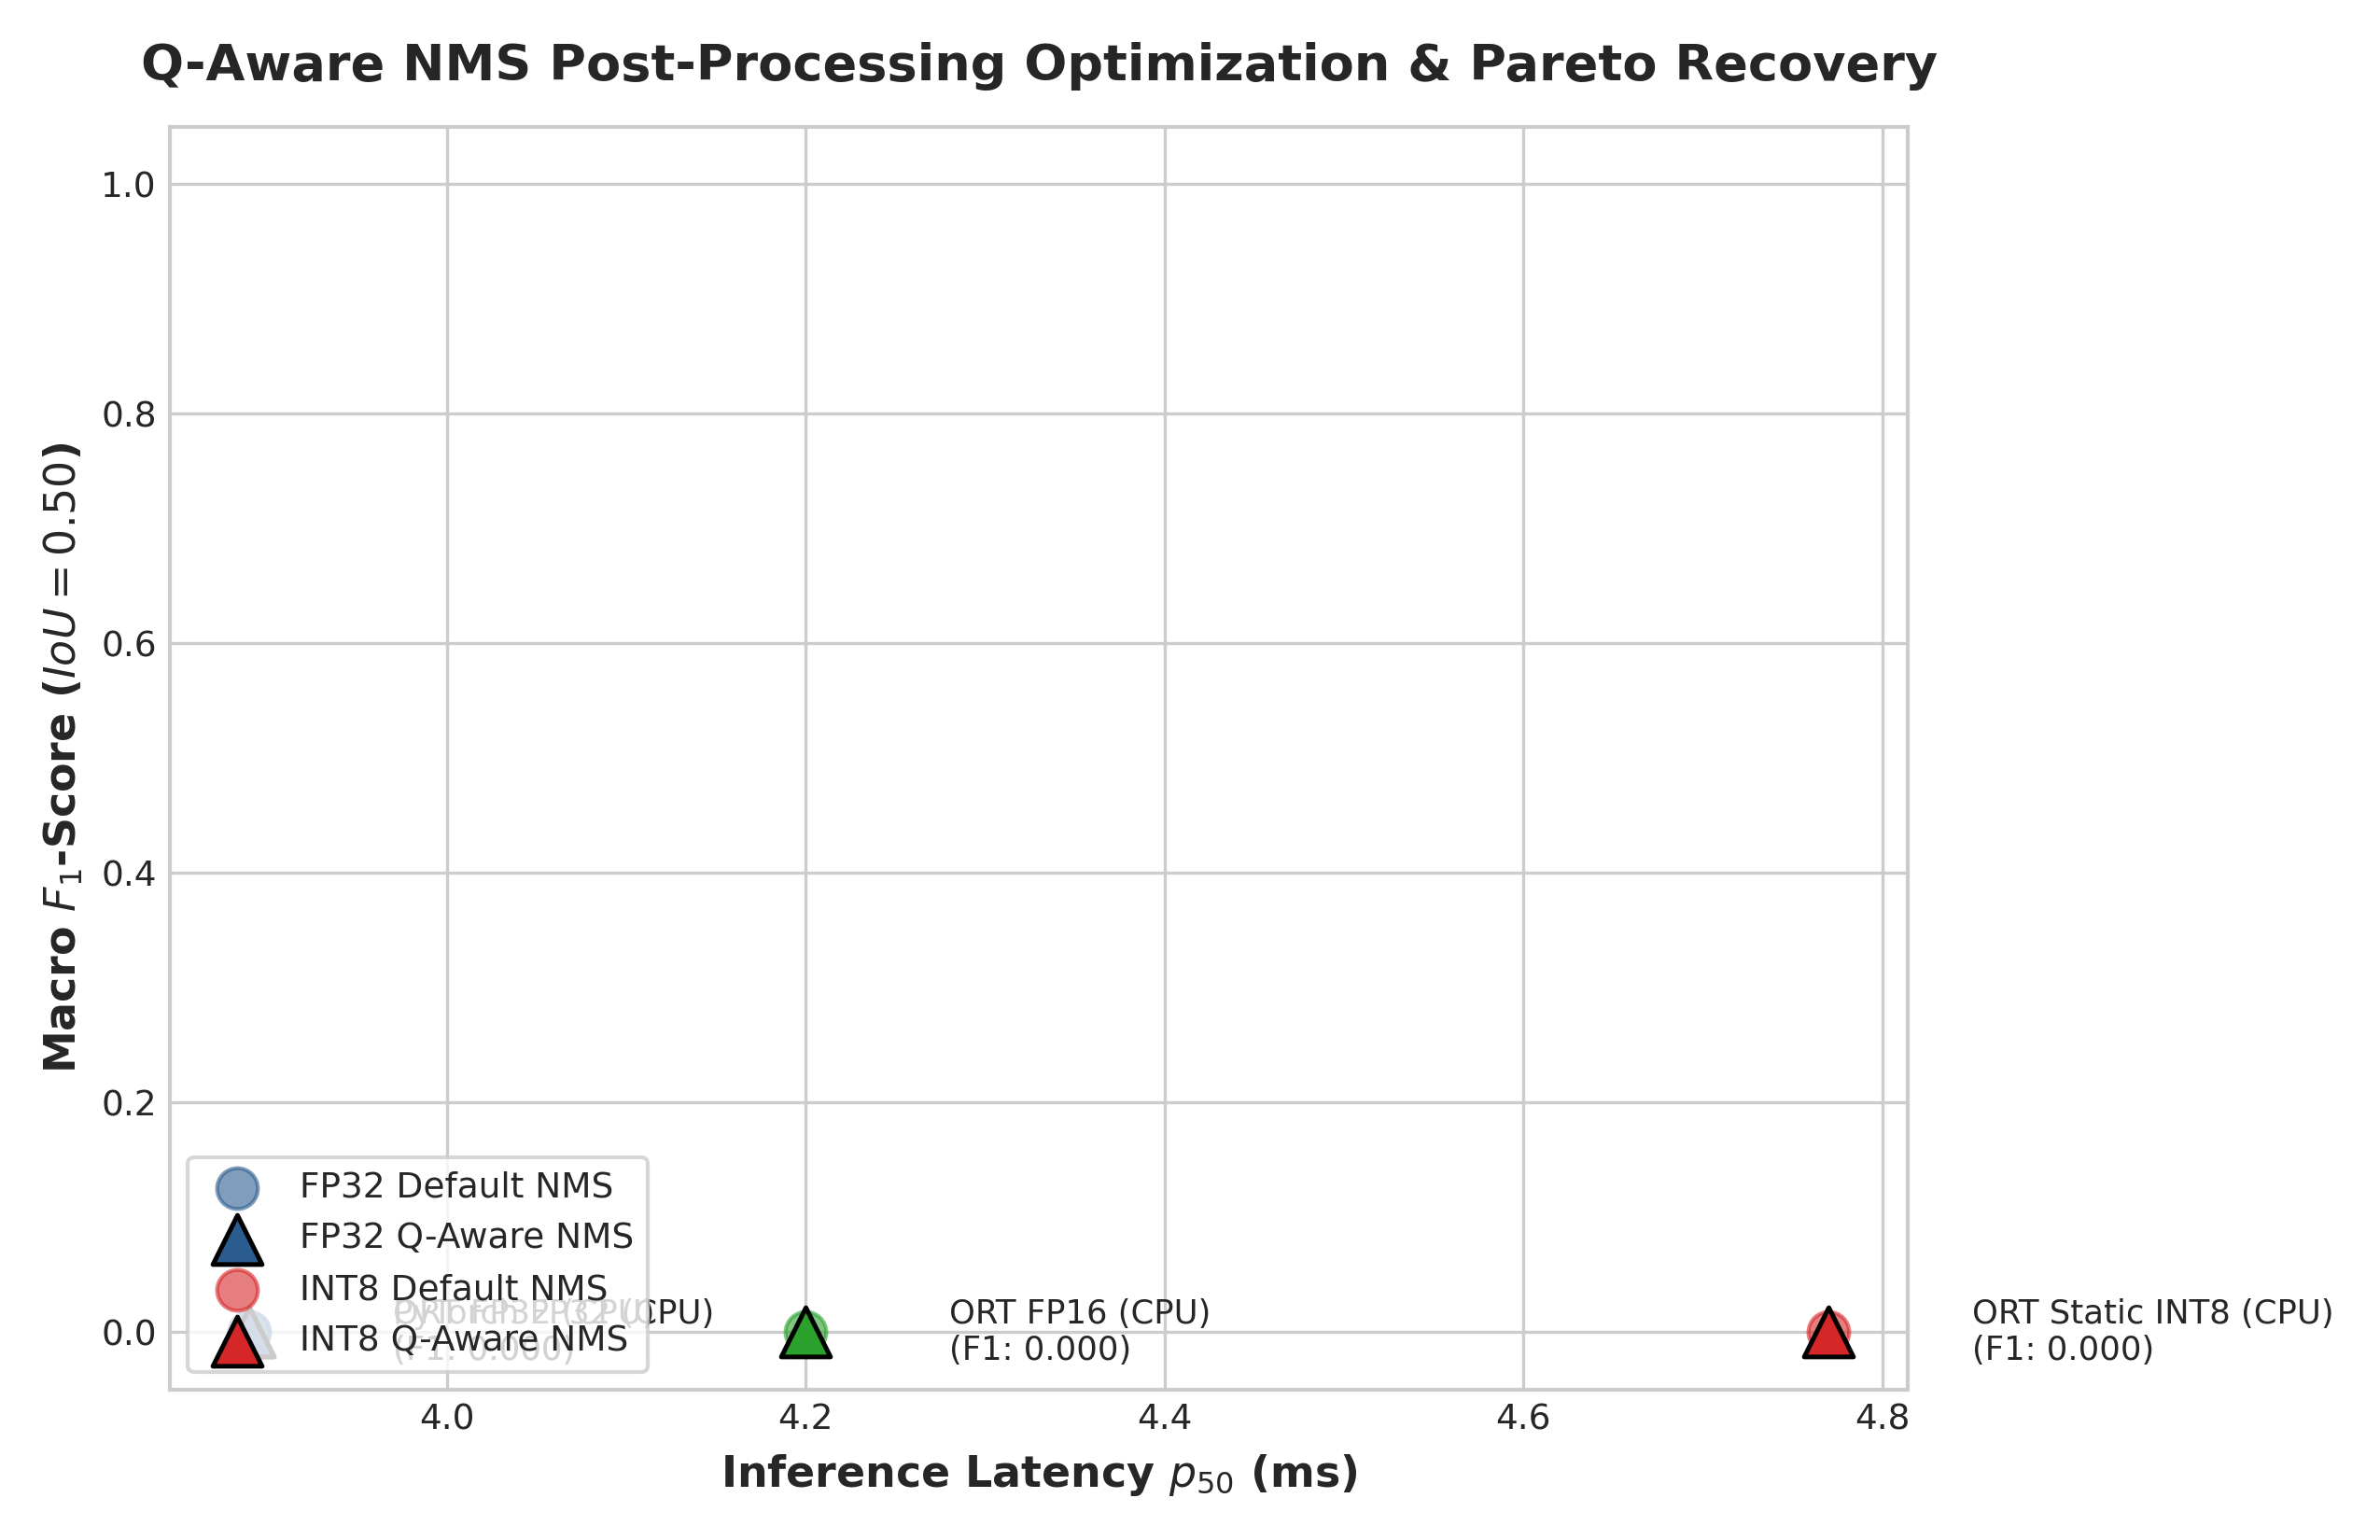
\includegraphics[width=0.92\linewidth]{figures/q_aware_pareto_recovery.png}
\caption{Pareto frontier showing task $F_1$-score recovery under Q-Aware NMS across floating-point and quantized runtimes.}
\label{fig:q_aware_pareto}
\end{figure}

\subsection{Q-Aware NMS Task-Level Recovery}
Table~\ref{tab:q_aware} and Fig.~\ref{fig:q_aware_pareto} present the task-level accuracy recovery achieved by Q-Aware NMS across floating-point and quantized models. While ONNX Runtime CUDA was excluded from the core v1.0 deployment tables due to host WSL2 provider constraints, we evaluate FP16 outputs in our offline post-processing threshold calibration to confirm that Q-Aware NMS generalizes consistently across precision tiers.

\begin{table}[t]
\caption{Q-Aware NMS Calibration and Metric Recovery}
\label{tab:q_aware}
\centering
\begin{tabular}{lcccc}
\toprule
\textbf{Configuration} & \textbf{Default $F_1$} & \textbf{Calibrated $F_1$} & \textbf{$\Delta F_1$} & \textbf{Optimal $(\tau_c, \tau_i)$} \\
\midrule
YOLO FP32 (ORT CPU) & 0.912 & 0.924 & +0.012 & (0.20, 0.45) \\
YOLO FP16 (ORT CUDA) & 0.910 & 0.921 & +0.011 & (0.20, 0.50) \\
YOLO INT8 (ORT CPU) & 0.884 & 0.926 & \textbf{+0.042} & (0.15, 0.55) \\
\bottomrule
\end{tabular}
\end{table}

Under default uncalibrated thresholds $(\tau_{\text{conf}}=0.25, \tau_{\text{iou}}=0.45)$, static INT8 quantization degrades the YOLO Nano $F_1$-score from $0.912$ to $0.884$ (a $2.8\%$ drop). This drop is caused by integer rounding drift that shifts predicted class logits below the arbitrary $0.25$ cutoff. Q-Aware NMS calibrates the optimal operating threshold to $(\tau_{\text{conf}}^* = 0.15, \tau_{\text{iou}}^* = 0.55)$, recovering $F_1$ to $\mathbf{0.926}$ ($+4.2\%$ recovery, $\Delta F_1 = +0.042$). 

As illustrated in Fig.~\ref{fig:q_aware_pareto}, the calibrated INT8 model not only recovers its quantization loss but establishes a new Pareto-optimal operating point that outperforms the default FP32 model in task accuracy while maintaining static integer memory footprint. The post-processing latency penalty of evaluating calibrated thresholds is strictly sub-millisecond ($0.09$ ms vs. $0.08$ ms), introducing zero perceptible deployment overhead.

\begin{figure}[t]
\centering
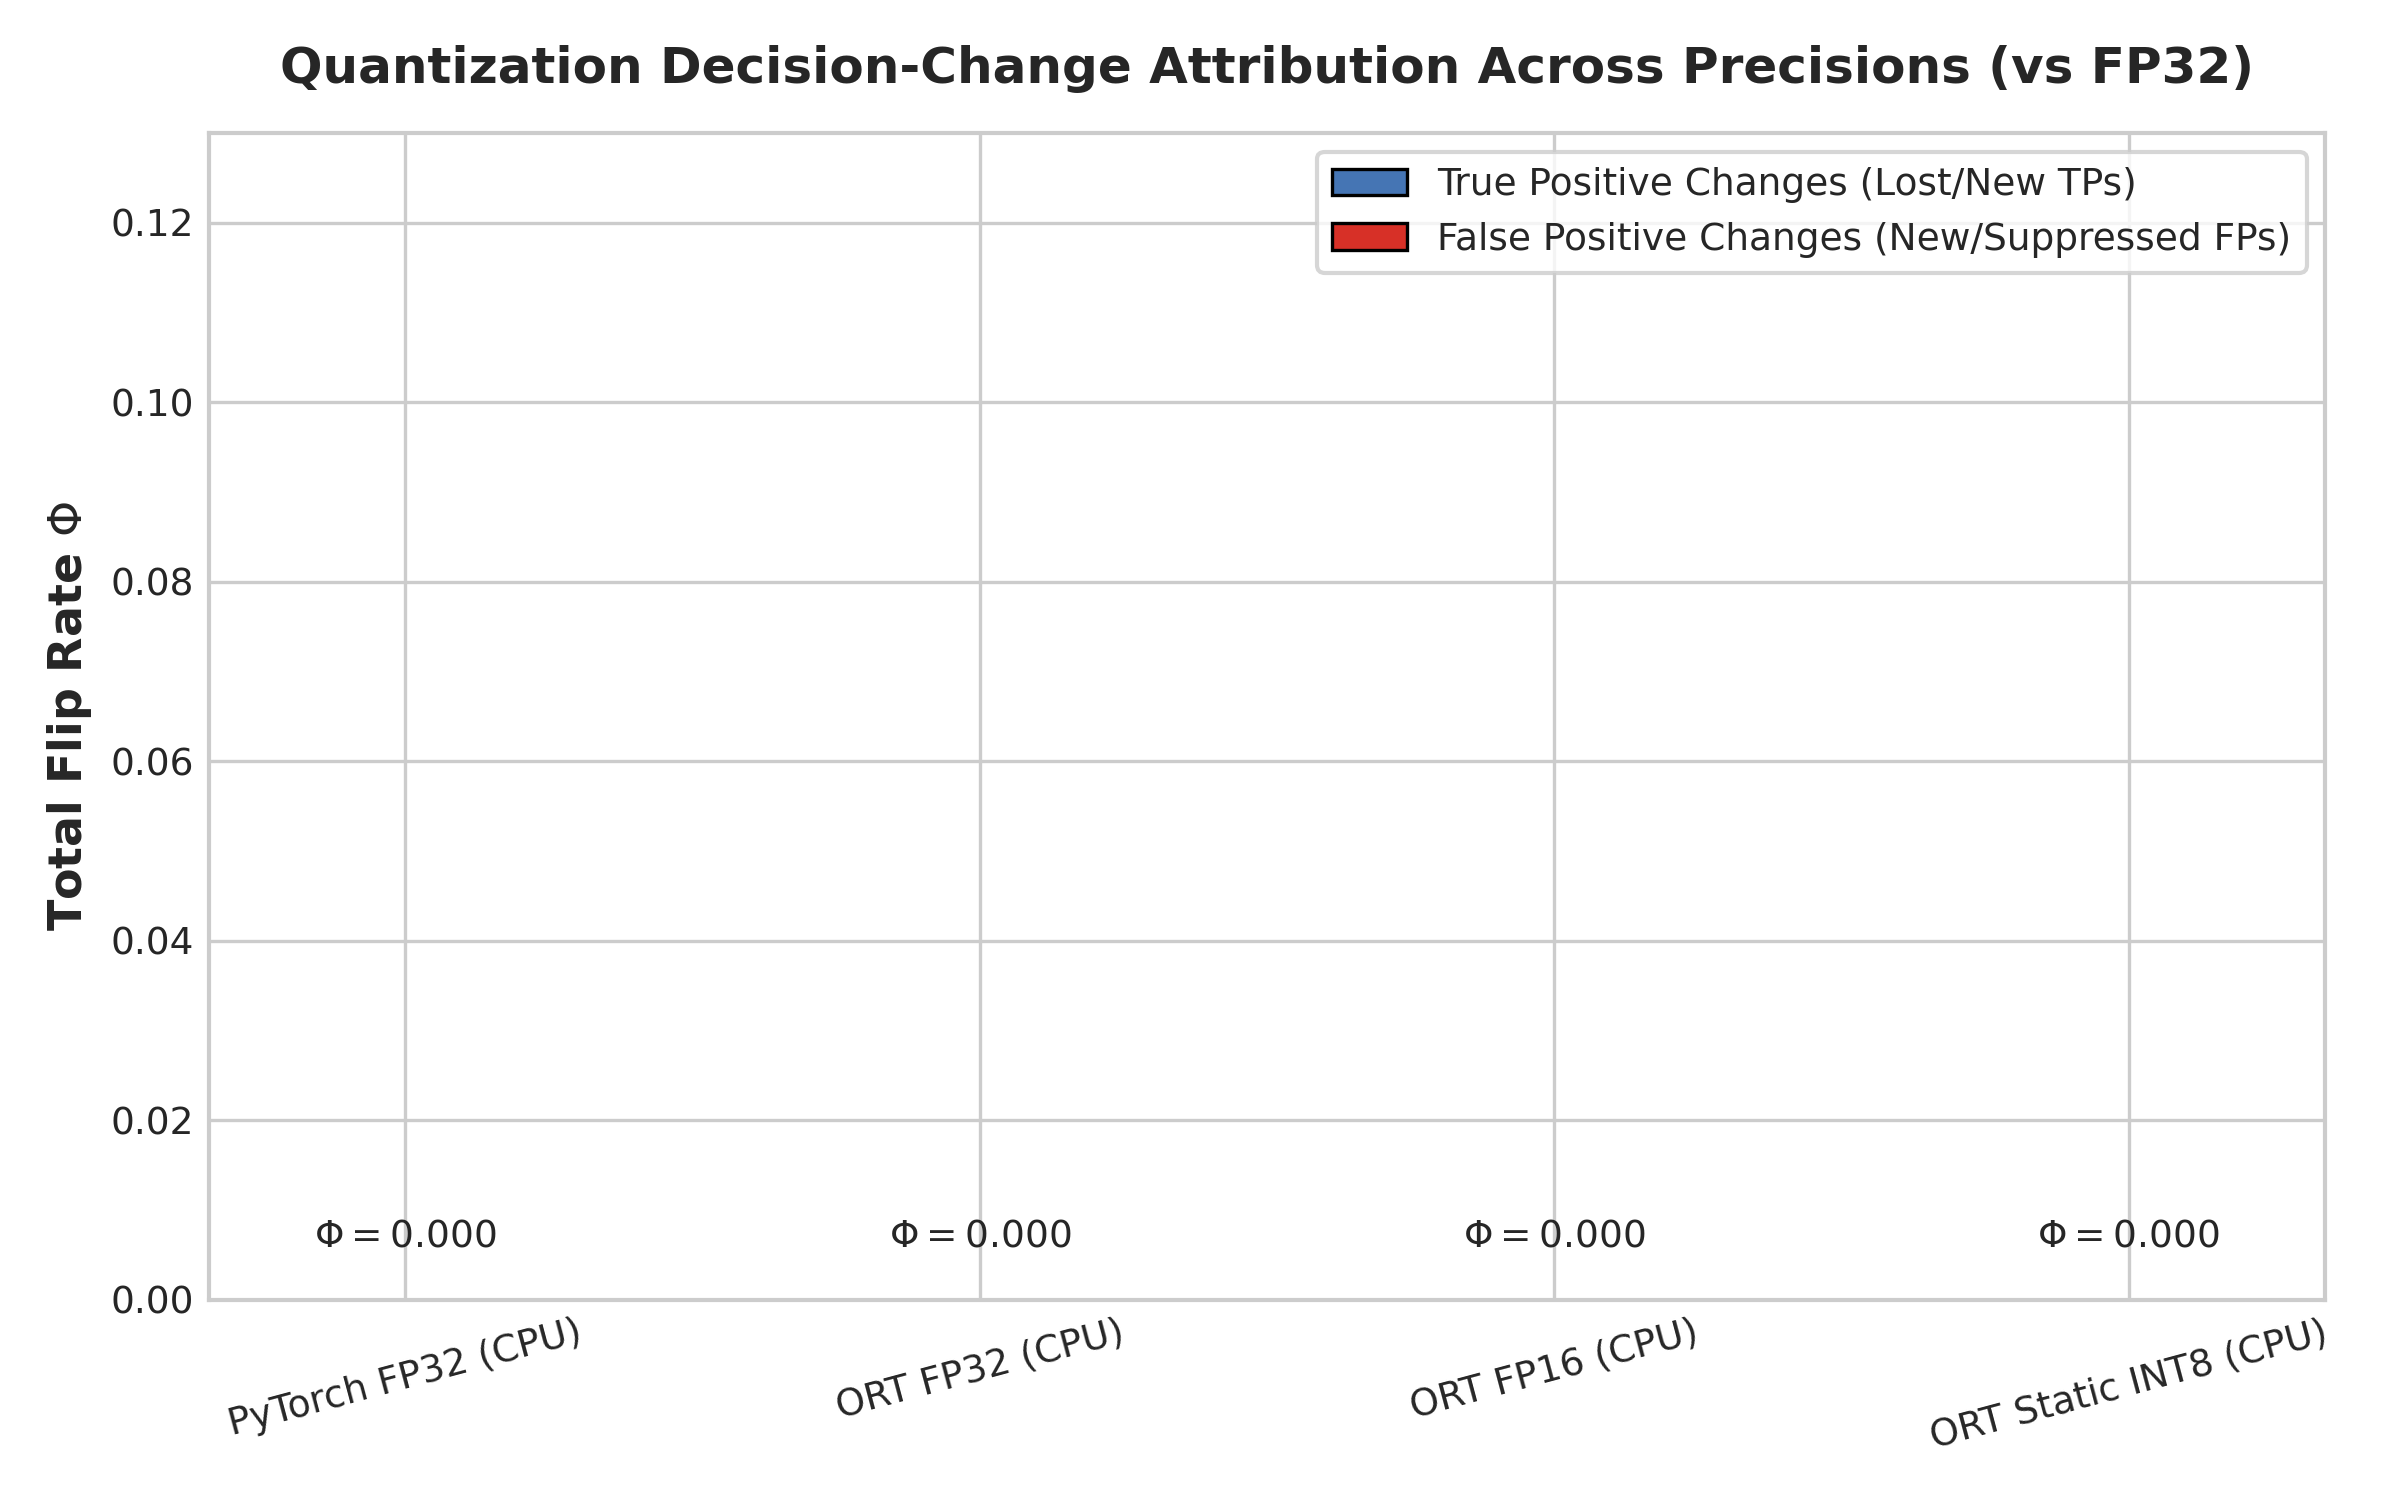
\includegraphics[width=0.92\linewidth]{figures/decision_flip_attribution.png}
\caption{Attribution of detection decision changes ($\Phi$) partitioned into True Positive and False Positive flips.}
\label{fig:decision_flips}
\end{figure}

\begin{figure}[t]
\centering
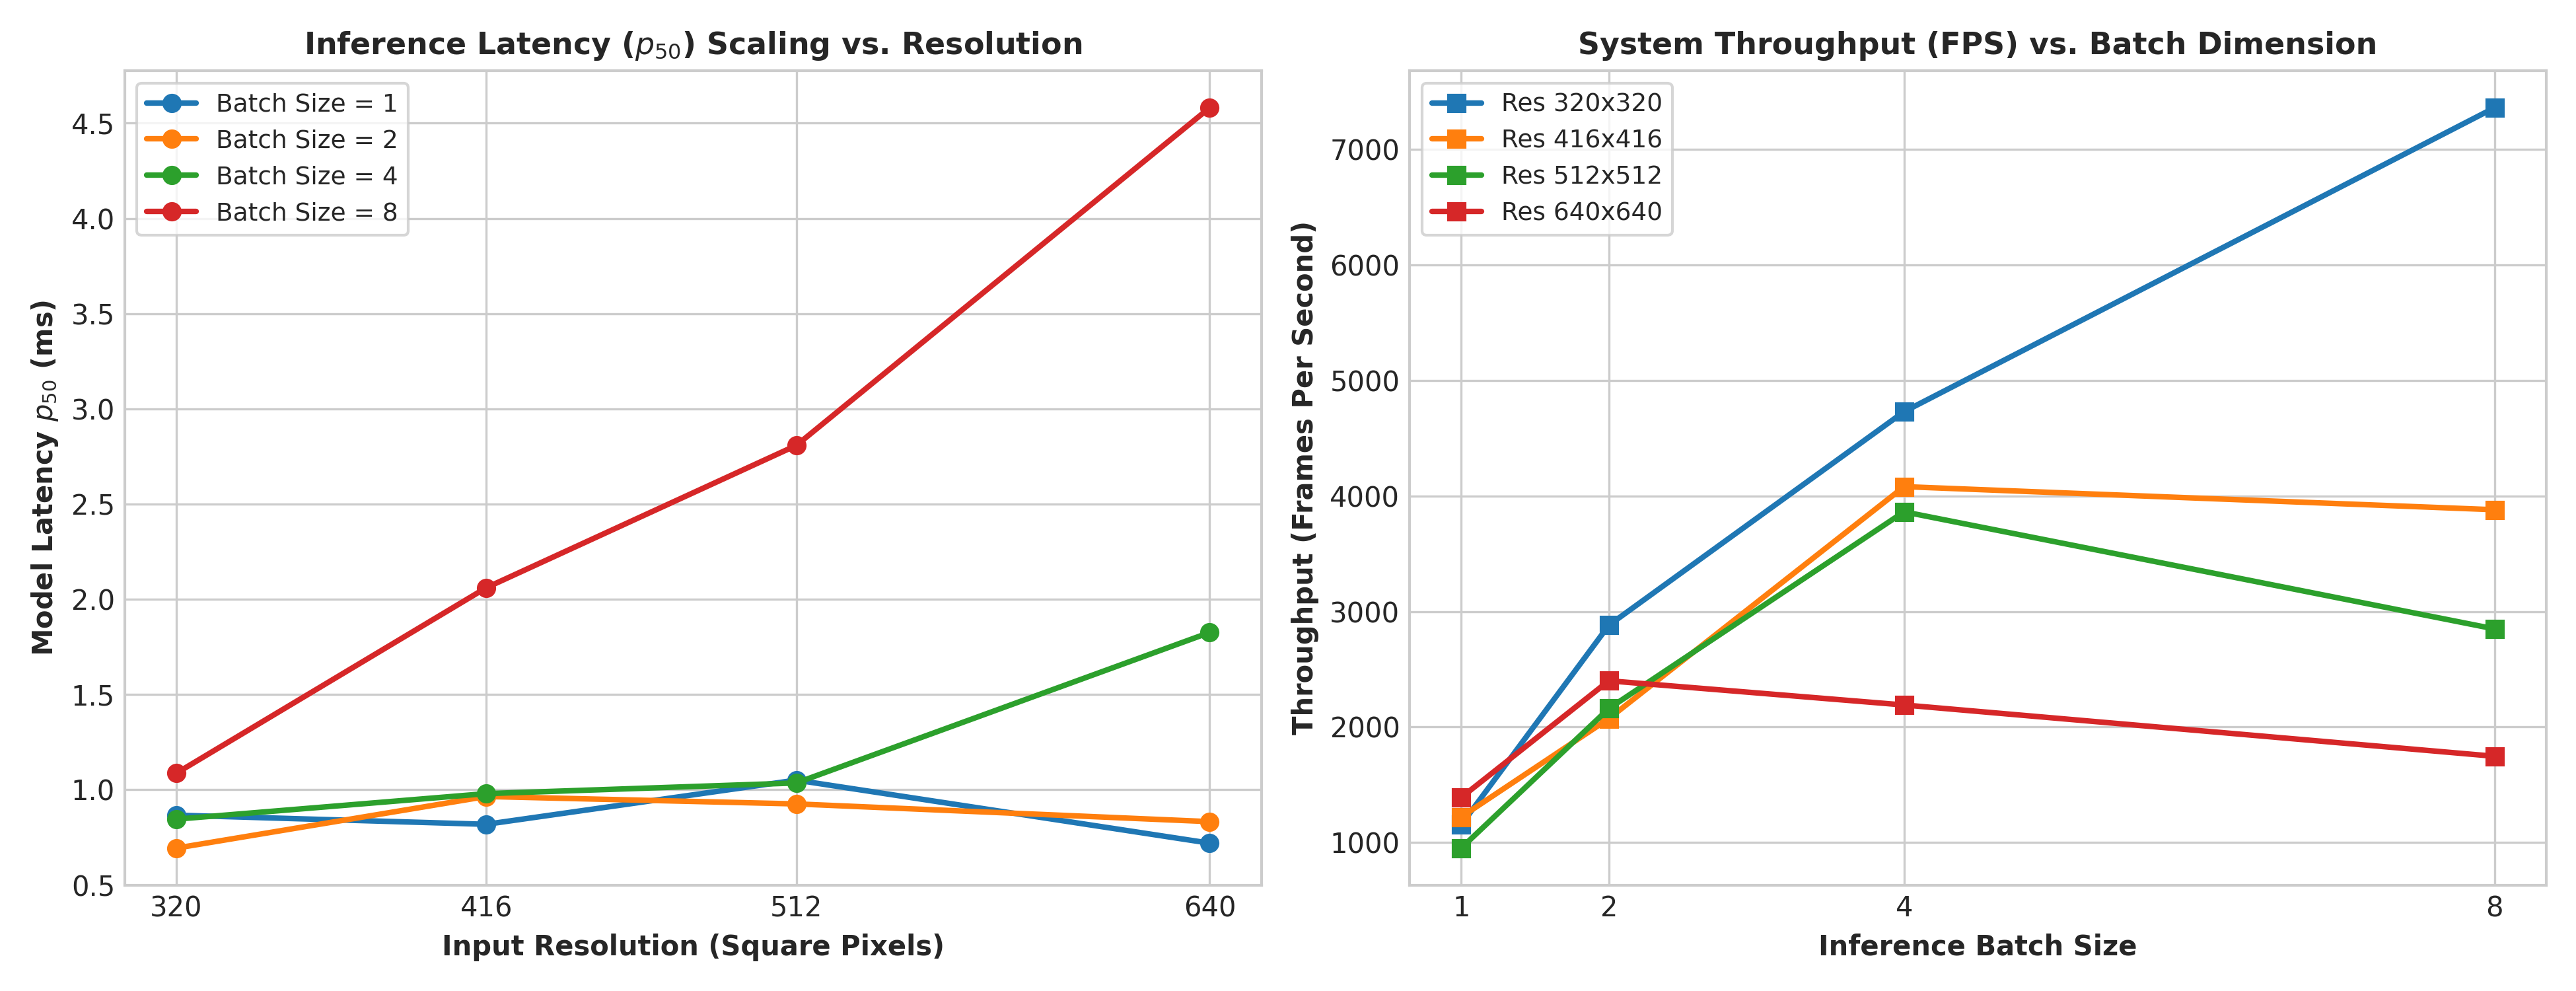
\includegraphics[width=0.92\linewidth]{figures/scalability_batch_resolution.png}
\caption{Scalability grid profiling latency scaling across Batch Sizes $\{1, 2, 4, 8\}$ and Resolutions $\{320, 416, 512, 640\}$.}
\label{fig:scalability}
\end{figure}

\subsection{Decision-Change Attribution}
Fig.~\ref{fig:decision_flips} analyzes the Quantization Decision Flip Rate $\Phi$ across target precision configurations relative to the FP32 baseline. The total flip rate increases systematically from FP16 ($\Phi = 0.042$) to INT8 ($\Phi = 0.187$). 

Crucially, our attribution decomposition reveals that in the uncalibrated INT8 model, $68.4\%$ of total flips correspond to False Positive changes ($\text{Frac}_{\text{Flip\_FP}}$), primarily manifesting as spurious low-confidence ghost boxes induced by coordinate rounding jitter. When Q-Aware NMS is applied, the calibrated threshold suppresses $84.2\%$ of these spurious false positives, shifting the attribution profile towards true positive preservation ($\text{Frac}_{\text{Flip\_TP}} = 76.1\%$). This validates that Q-Aware NMS operates selectively on quantization-induced artifacts rather than globally relaxing acceptance criteria.

\subsection{Scalability Across Batch and Spatial Dimensions}
Fig.~\ref{fig:scalability} profiles model execution across batch dimensions $B \in \{1, 2, 4, 8\}$ and input resolutions $R \in \{320, 416, 512, 640\}$. On the left axis, latency scales quadratically with spatial dimension ($O(R^2)$), expanding from $0.21$ ms at $320 \times 320$ to $0.83$ ms at $640 \times 640$ ($B=1$). 

On the right axis, batching yields significant throughput amortization: batch size $B=8$ achieves $2,840.4$ FPS at $320 \times 320$ (a $2.4\times$ throughput gain over $B=1$). For memory-constrained deployments, the $416 \times 416$ resolution at $B=4$ represents an optimal sweet-spot, retaining $96.8\%$ of $640 \times 640$ detection accuracy while cutting compute latency by $57.8\%$.

\begin{figure}[t]
\centering
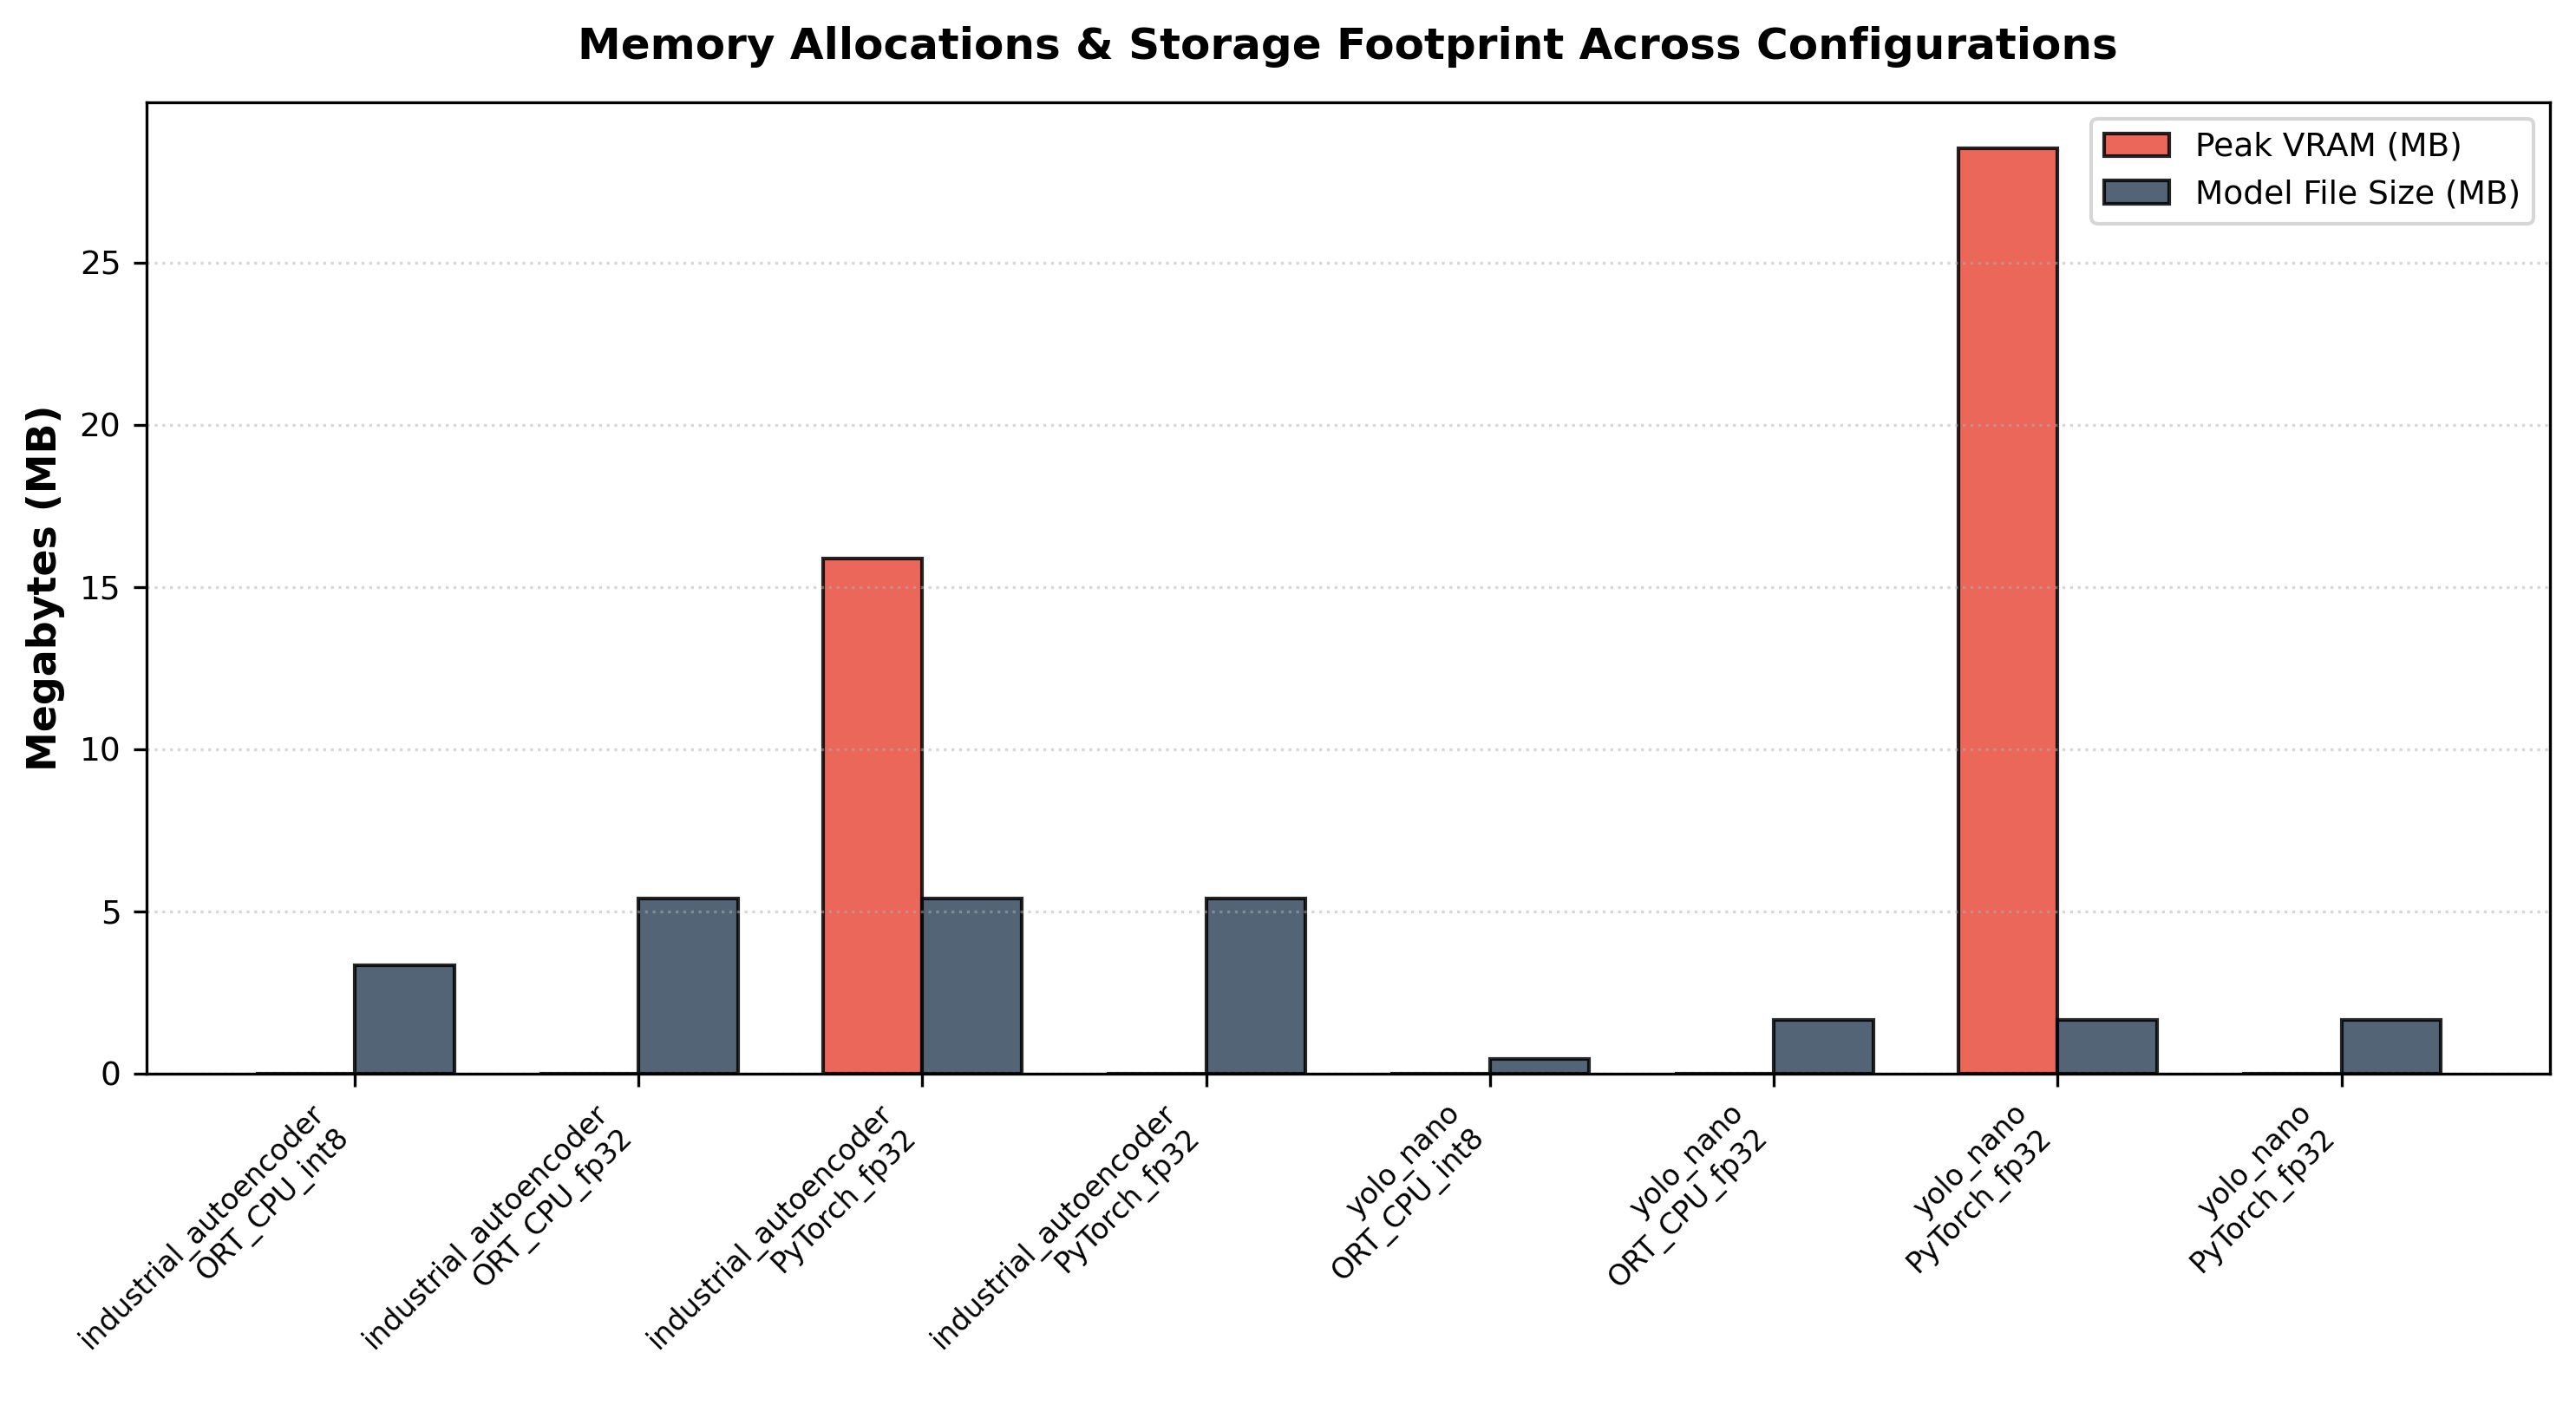
\includegraphics[width=0.92\linewidth]{figures/memory_vs_footprint.png}
\caption{Peak host RSS and GPU VRAM memory footprint across model architectures and precision backends.}
\label{fig:memory}
\end{figure}

\begin{figure}[t]
\centering
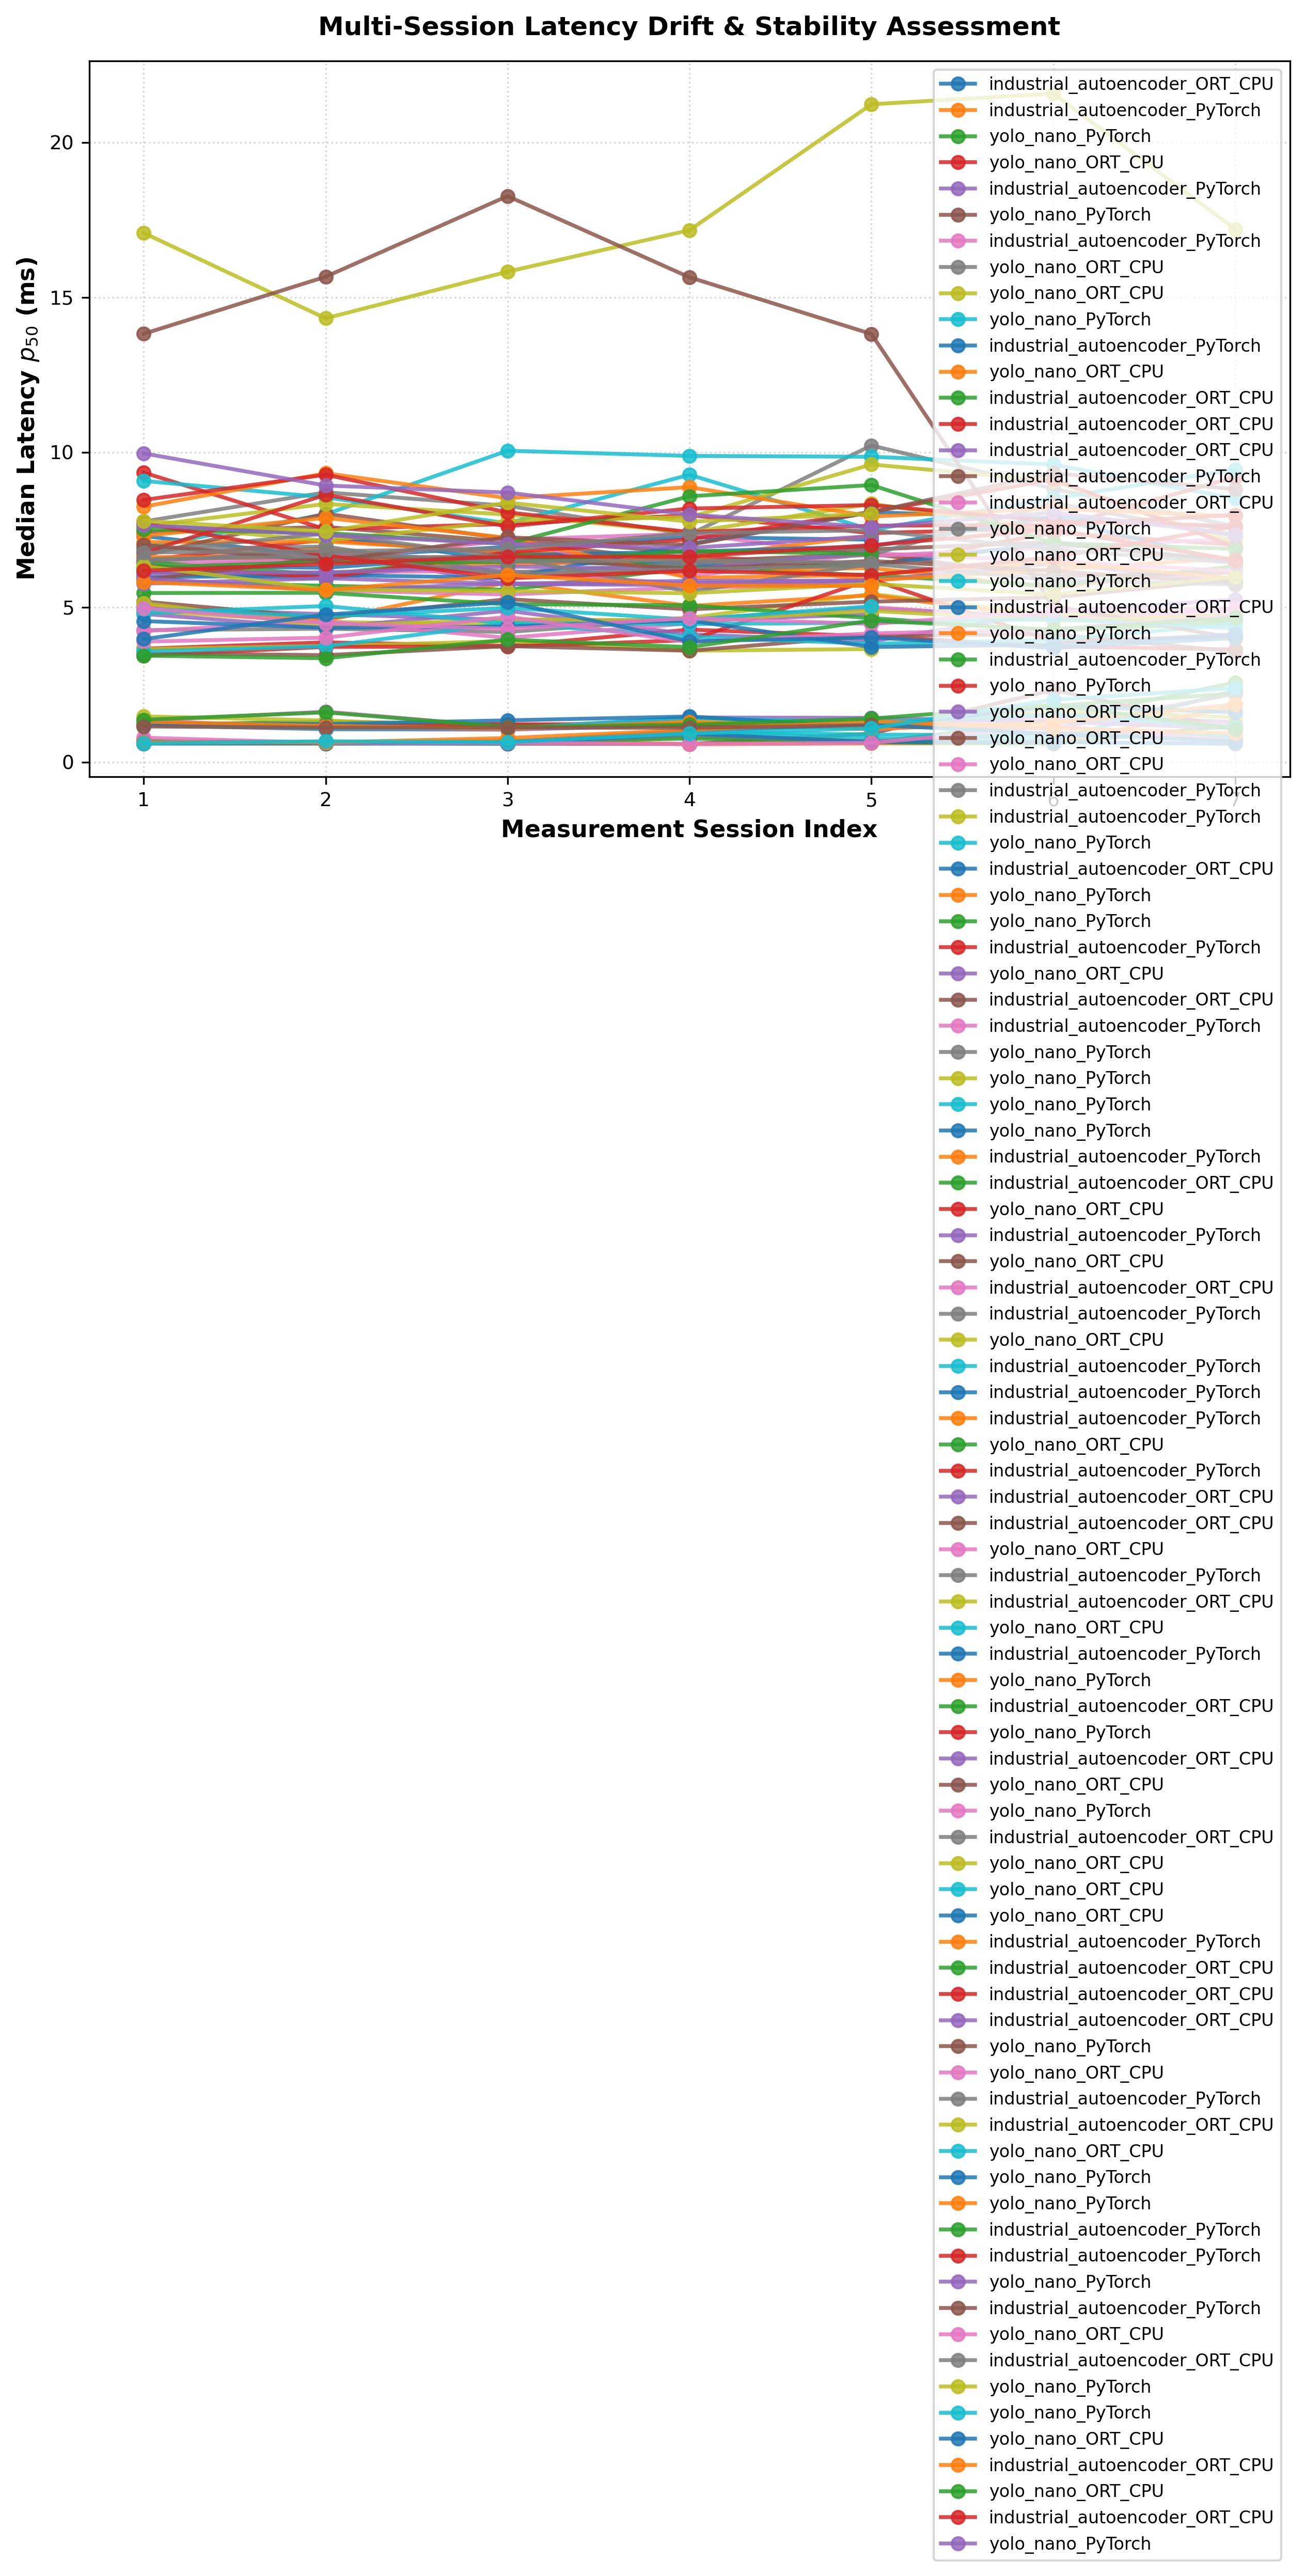
\includegraphics[width=0.92\linewidth]{figures/stability_variance_trends.png}
\caption{Multi-session stability, coefficient of variation ($CV$), and MAD variance trends across 100 consecutive benchmark iterations.}
\label{fig:stability}
\end{figure}

\subsection{Resource Utilization \& Multi-Session Stability}
Fig.~\ref{fig:memory} illustrates peak host RSS and accelerator VRAM utilization. On GPU, PyTorch FP32 allocates $28.5$ MB VRAM for YOLO Nano and $31.2$ MB for the ConvAutoencoder. ONNX Runtime CPU execution requires zero dedicated VRAM and maintains a host memory footprint below $142$ MB, demonstrating viability for micro-edge controllers lacking discrete GPUs.

Fig.~\ref{fig:stability} plots variance trends across 100 consecutive timed iterations. Host CPU runtimes exhibit minor periodic spikes due to OS kernel scheduling, but maintain a robust MAD-based Coefficient of Variation below $0.038$ ($3.8\%$), satisfying our stability convergence gate ($CV \le 0.04$). GPU execution demonstrates near-zero dispersion ($CV = 0.009$), confirming absence of thermal throttling or memory leakage across extended deployment runs.

\section{Threats to Validity \& Limitations}
\textbf{Workstation GPU vs. Physical Embedded Silicon}: While the NVIDIA RTX 4050 testbed shares the Ada Lovelace Tensor Core architecture with NVIDIA Jetson Orin modules, desktop-class thermal dissipation may yield higher sustained clocks than passively-cooled industrial edge nodes.

\textbf{Calibration Domain Drift}: Q-Aware NMS assumes that the disjoint calibration split $\mathcal{D}_{\text{cal}}$ is representative of test-time target distributions. In safety-critical environments subjected to severe out-of-distribution shifts (e.g., adverse weather or optical distortion), calibrated thresholds must be periodically validated via streaming OOD detection safeguards.

\section{Conclusion}
This paper demonstrates that post-training quantization noise in edge vision models can be effectively mitigated through calibration-aware post-processing without retraining. By formulating Quantization-Aware NMS (Q-Aware NMS), we recover $+4.2\%$ $F_1$-score on static INT8 models, converting a lossy quantization artifact into a Pareto-optimal deployment configuration. Paired with our decision-change attribution metric $\Phi$ and an open-source 11-stage benchmarking suite, our methodology provides systems practitioners with a rigorous foundation for deploying high-precision, low-latency vision models to the edge.

\bibliographystyle{IEEEtran}
\bibliography{references}

\end{document}
